

\section{virtual memory}

\subsection{address spaces}

\usetikzlibrary{arrows.meta,calc,fit,patterns,positioning,shapes.multipart}
\begin{frame}{program memory}
\begin{tikzpicture}
\tikzset{
    mylabel/.style={font=\ttfamily},
    mybox/.style={draw,rectangle,minimum width=5cm,fill=white},
    myhigh/.style={draw,rectangle,line width=1mm, draw=blue!80!black,opacity=.3},
}
\node[mybox,minimum height=1cm,pattern=north west lines,pattern color=black!5!white] (kernel) {Used by OS};
\begin{pgfonlayer}{bg}
\node[right=1mm of kernel.north east,mylabel] (topLabel) {0xFFFF FFFF FFFF FFFF};
\node[right=1mm of kernel.south east,mylabel] {0xFFFF 8000 0000 0000};
\end{pgfonlayer}
\node[mybox, minimum height=.5cm, below=1cm of kernel] (stack) {Stack};
\begin{pgfonlayer}{bg}
\node[right=1mm of stack.north east,mylabel] {0x7F\ldots{}};
\end{pgfonlayer}
\node[mybox, minimum height=.5cm, below=1cm of stack] (heap) {Heap / other dynamic};
\node[mybox, minimum height=.5cm, below=0mm of heap] (data) {Writable data};
\node[mybox, minimum height=.5cm, below=0mm of data] (sdata) {Code + Constants};
\begin{pgfonlayer}{bg}
\node[right=1mm of sdata.south east,mylabel] (bottomLabel) {0x0000 0000 0040 0000};
\end{pgfonlayer}
\coordinate (memBottom) at ($(sdata.south east) + (0mm, -2mm)$);
\begin{pgfonlayer}{bg}
\draw[pattern=north west lines, pattern color=black!40!white] (kernel.north west) rectangle (memBottom);
\end{pgfonlayer}
\end{tikzpicture}
\end{frame}

\begin{frame}{address spaces}
\begin{itemize}
\item illuision of \myemph{dedicated memory}
\end{itemize}
\begin{tikzpicture}
\tikzset{
    every node/.style={font=\small},
}
\node[align=center] (progAAddr) {Process A \\ addresses};
\node[below=1cm of progAAddr,align=center] (progBAddr) {Process B \\ addresses};
\node[draw, right=3cm of progAAddr,align=center] (translationA) { mapping \\ (set by OS) };
\node[draw, right=3cm of progBAddr,align=center] (translationB) { mapping \\ (set by OS) };
\node[draw,rectangle split, rectangle split parts=6, anchor=north west,label={north:real memory}] (mem) at ([xshift=3.5cm]translationA.north east) {
    \nodepart{one}
    Process A code 
    \nodepart{two}
    Process B code
    \nodepart{three}
    Process A data
    \nodepart{four}
    Process B data
    \nodepart{five}
    OS data
    \nodepart{six}
    \ldots
};
\draw[-Latex,green,thick] (progAAddr) -- (translationA) (translationA.east) -- (mem.one west);
\draw[-Latex,green,thick] (translationA.east) -- (mem.three west);
\draw[-Latex,blue,thick] (progBAddr) -- (translationB) (translationB.east) -- (mem.two west);
\draw[-Latex,blue,thick] (translationB.east) -- (mem.four west);
\node[thick,draw,anchor=north west] (error) at ([yshift=-.5cm]mem.south west) {trigger exception};
\draw[-Latex,green,thick] (translationA.east) -- (error.west);
\draw[-Latex,blue,thick] (translationB.east) -- (error.west);
\draw[-Latex,green,ultra thick,dotted] (translationA.east) -- (mem.five west);
\draw[-Latex,blue,ultra thick,dotted] (translationB.east) -- (mem.five west);
\draw[-Latex,ultra thick,dotted] ([xshift=-3cm,yshift=-.5cm]translationB.south) -- ([xshift=-2cm,yshift=-.5cm]translationB.south)
    node[right] {= kernel-mode only};
\begin{visibleenv}<2>
    \node[fill=red,fill opacity=0.1,draw=red,ultra thick,fit=(translationA) (translationB),label={[red]north:chose one during context switch}] {};
\end{visibleenv}
\end{tikzpicture}
\end{frame}

  % FIXME: some duplication with memProtect exceptions slides
\usetikzlibrary{arrows.meta,fit}

\begin{frame}{address spaces}
\begin{itemize}
\item illusion of \myemph{dedicated memory}
\end{itemize}
\myalttext{
\begin{tikzpicture}
\tikzset{
    every node/.style={font=\small},
}
\node[align=center] (progAAddr) {Process A \\ addresses};
\node[below=1cm of progAAddr,align=center] (progBAddr) {Process B \\ addresses};
\node[draw, right=3cm of progAAddr,align=center] (translationA) { mapping \\ (set by OS) };
\node[draw, right=3cm of progBAddr,align=center] (translationB) { mapping \\ (set by OS) };
\node[draw,rectangle split, rectangle split parts=6, anchor=north west,label={north:real memory}] (mem) at ([xshift=3.5cm]translationA.north east) {
    \nodepart{one}
    Process A code 
    \nodepart{two}
    Process B code
    \nodepart{three}
    Process A data
    \nodepart{four}
    Process B data
    \nodepart{five}
    OS data
    \nodepart{six}
    \ldots
};
\draw[-Latex,green,thick] (progAAddr) -- (translationA) (translationA.east) -- (mem.one west);
\draw[-Latex,green,thick] (translationA.east) -- (mem.three west);
\draw[-Latex,blue,thick] (progBAddr) -- (translationB) (translationB.east) -- (mem.two west);
\draw[-Latex,blue,thick] (translationB.east) -- (mem.four west);
\node[thick,draw,anchor=north west] (error) at ([yshift=-.5cm]mem.south west) {trigger exception};
\draw[-Latex,green,thick] (translationA.east) -- (error.west);
\draw[-Latex,blue,thick] (translationB.east) -- (error.west);
\draw[-Latex,green,ultra thick,dotted] (translationA.east) -- (mem.five west);
\draw[-Latex,blue,ultra thick,dotted] (translationB.east) -- (mem.five west);
\draw[-Latex,ultra thick,dotted] ([xshift=-3cm,yshift=-.5cm]translationB.south) -- ([xshift=-2cm,yshift=-.5cm]translationB.south)
    node[right] {= kernel-mode only};
\begin{visibleenv}<2>
    \node[fill=red,fill opacity=0.1,draw=red,ultra thick,fit=(translationA) (translationB),label={[red]north:chose one during context switch}] {};
\end{visibleenv}
\end{tikzpicture}
}{Diagram showing processes A and B have different mappings from virtual (program) to physical (real) addresses set by the OS.
The mapping can also specifies that some addresses trigger exceptions or are usable in kernel mode only.}
\end{frame}


\subsection{address translation overview}
\usetikzlibrary{arrows.meta,calc,positioning,shapes.multipart}
\begin{frame}{address translation}
\myalttext{
\begin{tikzpicture}
\tikzset{
    every node/.style={font=\small},
}
\node[align=center,alt=<2>{draw=red,very thick,fill=red!10}{}] (progAAddr) {Process A \\ addresses \\ \myemph<3>{``virtual''}};
\begin{visibleenv}<2>
\node[align=left,below=.5cm of progAAddr] {\myemph{every address accessed} \\ instructions \textit{and} data};
\end{visibleenv}
%\node[below=1cm of progAAddr,align=center] (progBAddr) {Process B \\ addresses};
\node[draw, right=3cm of progAAddr,align=center,alt=<4>{draw=red,very thick,fill=red!10}] (translationA) { mapping \\ (set by OS) };
\begin{visibleenv}<4>
\node[align=left,below=.5cm of translationA] {stored in processor? \\ format?};
\end{visibleenv}
%\node[draw, right=3cm of progBAddr,align=center] (translationB) { mapping \\ (set by OS) };
\node[draw,rectangle split, rectangle split parts=6, anchor=north west,label={[align=center]north:real memory\\\myemph<3>{``physical''}}] (mem) at ([xshift=3cm]translationA.north east) {
    \nodepart{one}
    Process A code 
    \nodepart{two}
    Process B code
    \nodepart{three}
    Process A data
    \nodepart{four}
    Process B data
    \nodepart{five}
    OS data
    \nodepart{six}
    \ldots
};
\draw[-Latex,green,thick] (progAAddr) -- (translationA) (translationA.east) -- (mem.one west);
\draw[-Latex,green,thick] (translationA.east) -- (mem.three west);
%\draw[-Latex,blue,thick] (progBAddr) -- (translationB) (translationB.east) -- (mem.two west);
%\draw[-Latex,blue,thick] (translationB.east) -- (mem.four west);
%\node[thick,red,draw,anchor=north west] (error) at ([yshift=-.5cm]mem.south west) {trigger error};
%\draw[-Latex,green,thick] (translationA.east) -- (error.west);
%\draw[-Latex,blue,thick] (translationB.east) -- (error.west);
%\draw[-Latex,green,ultra thick,dotted] (translationA.east) -- (mem.five west);
%\draw[-Latex,blue,ultra thick,dotted] (translationB.east) -- (mem.five west);
\begin{visibleenv}<3>
\node[draw,thick,align=center,below=3cm of translationA] {
    program addresses are `virtual' \\
    real addresses are `physical' \\
    can be \myemph{different sizes}!
};
\end{visibleenv}
\end{tikzpicture}
}{%
    Diagram showing program addresses (program and data) being converted to real addresses using a mapping set by the OS.
    The program addresses are called "virtual" and the real addresses are called "physical".
}
\end{frame}


\subsection{simple paging with four pages}
\usetikzlibrary{arrows.meta,calc,fit,matrix,patterns,positioning}
\begin{frame}{toy program memory}
\begin{tikzpicture}
\tikzset{
    >=Latex,
    addr/.style={font=\fontsize{12}{13}\selectfont\tt},
}
\draw[very thick] (0, 0) rectangle (4, 4);
\foreach \x in {1,2,3} {
    \draw[thick] (0, \x) -- (4, \x);
}
\node at (2, 0.5) {code};
\node at (2, 1.5) {data/heap};
\node at (2, 2.5) {empty/more heap?};
\node at (2, 3.5) {stack};
\draw[<-,thick] (0,0.0)  -- ++ (-.5cm,0cm) node [left,addr] {\myemph<4>{00} \myemph<5>{0000 0000} = 0x000};
\draw[<-,thick] (0,1.0)  -- ++ (-.5cm,0cm) node [left,addr] {\myemph<4>{01} \myemph<5>{0000 0000} = 0x100};
\draw[<-,thick] (0,2.0)  -- ++ (-.5cm,0cm) node [left,addr] {\myemph<4>{10} \myemph<5>{0000 0000} = 0x200};
\draw[<-,thick] (0,3.0)  -- ++ (-.5cm,0cm) node [left,addr] {\myemph<4>{11} \myemph<5>{0000 0000} = 0x300};
\draw[<-,thick] (0,3.95)  -- ++ (-.5cm,0cm) node [left,addr] {\myemph<4>{11} \myemph<5>{1111 1111} = 0x3FF};
\begin{visibleenv}<2->
\foreach \x/\y in {0/green,1/blue,2/orange,3/yellow} {
    \fill[\y,opacity=0.10] (0, \x) rectangle ($(0, \x) + (4, 1)$);
    \node[anchor=west] at ($(0, \x) + (4, 0.5)$) {virtual page\# \myemph<4>{\x}};
}
\end{visibleenv}
\begin{visibleenv}<3>
\node[draw=red,thick,fill=white,align=left] at (0, -2) {
    divide memory into \myemph{pages} ($2^8$ bytes in this case) \\
    ``virtual'' = addresses the program sees
};
\end{visibleenv}
\begin{visibleenv}<4>
\node[draw=red,thick,fill=white,align=left] at (0, -2) {
    \myemph{page number} is upper bits of address \\
    (because page size is power of two)
};
\end{visibleenv}

\begin{visibleenv}<5>
\node[draw=red,thick,fill=white,align=left] at (0, -2) {
    rest of address is called \myemph{page offset}
};
\end{visibleenv}
\end{tikzpicture}
\end{frame}

\begin{frame}{toy physical memory}
\begin{tikzpicture}
\tikzset{
    >=Latex,
    addr/.style={font=\small\tt},
    y=0.8cm,
}
\node[anchor=south,align=center]at (2, 4) {program memory \\ \myemph{virtual addresses}};
\draw[very thick] (0, 0) rectangle (4, 4);
\foreach \x in {1,2,3} {
    \draw[thick] (0, \x) -- (4, \x);
}
\begin{scope}[every node/.style={font=\fontsize{10}{11}\selectfont\tt}]
\node[align=left] at (2, 0.5) {00 0000 0000 to \\ 00 1111 1111};
\node[align=left] at (2, 1.5) {01 0000 0000 to \\ 01 1111 1111};
\node[align=left] at (2, 2.5) {10 0000 0000 to \\ 10 1111 1111};
\node[align=left] at (2, 3.5) {11 0000 0000 to \\ 11 1111 1111};
\end{scope}
\foreach \x/\y in {0/green,1/blue,2/orange,3/yellow} {
    \fill[\y,opacity=0.10] (0, \x) rectangle ($(0, \x) + (4, 1)$);
}
\begin{scope}[xshift=6.5cm]
\node[overlay,anchor=south,align=center]at (2, 8) {real memory \\ \myemph{physical addresses}};
\draw[very thick] (0, 0) rectangle (4, 8);
\foreach \x in {1,2,3,...,7} {
    \draw[thick] (0, \x) -- (4, \x);
}
\begin{scope}[every node/.style={font=\fontsize{10}{11}\selectfont\tt}]
\node[align=left] at (2, 0.5) {\myemph<2>{000} 0000 0000 to \\ \myemph<2>{000} 1111 1111};
\node[align=left] at (2, 1.5) {\myemph<2>{001} 0000 0000 to \\ \myemph<2>{001} 1111 1111};
\node[align=left] at (2, 7.5) {\myemph<2>{111} 0000 0000 to \\ \myemph<2>{111} 1111 1111};
\end{scope}
\begin{visibleenv}<2>
\node[anchor=west] at (4, 0.5) {physical page 0};
\node[anchor=west] at (4, 1.5) {physical page 1};
\node[anchor=west] at (4, 7.5) {physical page 7};
\end{visibleenv}
\end{scope}
\begin{visibleenv}<3->
\draw[thick,->] (4, 0.5) -- (6.5, 2.5);
\draw[thick,->] (4, 1.5) -- (6.5, 7.5);
\draw[thick,->] (4, 3.5) -- (6.5, 0.5);
\end{visibleenv}
\begin{visibleenv}<4->
\matrix[tight matrix,anchor=north,
    nodes={text width=3.4cm,minimum height=0.5cm},
    column 1/.style={nodes={draw=none,font=\tt}},
    column 2/.style={nodes={draw,thick,font=\tt}},
    row 1/.style={nodes={draw=none,font=\normalfont}}] (thePt) at (2, 9.0) {
    virtual page \# \& physical page \# \\
    00 \& 010 \normalfont (2) \\
    01 \& 111 \normalfont (7) \\
    10 \& \normalfont\it none \\
    11 \& 000 \normalfont (0) \\
};
\end{visibleenv}
\begin{visibleenv}<5>
\node[draw=red,fill=red,fill opacity=0.1,ultra thick,inner sep=0.5mm,fit=(thePt)] {};
    \node[overlay,red,anchor=south west,align=left] at ([xshift=0cm,yshift=-0.25cm]thePt.north east) {\bfseries page\\\bfseries table!};
\end{visibleenv}
\end{tikzpicture}
\end{frame}

\begin{frame}{toy page table lookup}
\begin{tikzpicture}
\tikzset{
    >=Latex,
}
\matrix[tight matrix,anchor=north west,
    nodes={text width=2cm,minimum height=0.6cm},
    column 1/.style={nodes={draw=none,font=\tt,align=right}},
    column 2/.style={nodes={draw,thick,font=\tt,text width=1.2cm,align=center}},
    column 3/.style={nodes={draw,thick,font=\tt, text width=3.5cm}},
    column 4/.style={nodes={draw,thick,font=\tt,visible on=<all:0>, text width=1cm}},
    column 5/.style={nodes={draw,thick,font=\tt,visible on=<all:0>, text width=1cm}},
    row 1/.style={nodes={draw=none,font=\normalfont}},
    ] (pt) at (0, 5) {
    virtual page \# \& valid? \& physical page \# \& read OK? \& write OK? \\
    00 \& 1 \& 010 \normalfont (2, code) \& 1 \& 0 \\
    01 \& 1 \& 111 \normalfont (7, data) \& 1 \& 1 \\
    10 \& 0 \& ??? \normalfont (ignored) \& 0 \& 0 \\
    11 \& 1 \& 000 \normalfont (0, stack) \& 1 \& 1 \\
};
\begin{visibleenv}<all:2->
\node[draw,fill=blue!10,alt=<all:4>{draw=red,fill=red!10,ultra thick}] (addrLeft) at (-1, 6.0) {\tt 01};
    \node[anchor=west,fill=green!10,alt=<all:6>{draw=red,fill=red!10,ultra thick}] (addrRest) at (addrLeft.east) {\tt 1101 0010 \normalfont};
\node[anchor=west] (addrDesc) at (addrRest.east) {--- address from CPU};
    \draw[->,very thick,draw=blue!50!black] (addrLeft.south) |- ([xshift=4ex]pt-3-1.west);
    \draw[->,thick] (pt-5-2.south) |- ++(-1cm,-1.5cm) -- ++(0cm,-.5cm) node[below] {trigger exception if 0?};
\draw[->,very thick,draw=blue!50!black] ([xshift=3ex]pt-5-3.south west) |- ++(2cm,-1cm)
    node[right,fill=blue!10,alt=<all:5>{draw=red,fill=red!10,ultra thick}] (newAddrLeft) {\tt 111};
    \node[anchor=west,fill=green!10,alt=<all:6>{draw=red,fill=red!10,ultra thick}] (newAddrRight) at (newAddrLeft.east) {\tt 1101 0010};
\draw[->,very thick,draw=green!50!black] (addrRest) |- ([xshift=1cm,yshift=.5cm]pt-1-3.north east) -| (newAddrRight);
    \node[inner sep=0mm,draw=black,thin,fit=(newAddrLeft) (newAddrRight)] (newAddrBox) {};
    \draw[->,very thick] (newAddrBox.south) -- ++(0cm,-.5cm) node[below] {to memory};
\end{visibleenv}
\begin{visibleenv}<all:2>
\node[inner sep=0mm,draw=red,ultra thick,fit=(pt-3-2) (pt-3-3)] {};
\end{visibleenv}
\begin{visibleenv}<all:3>
\node[inner sep=0mm,draw=red,ultra thick,fit=(pt-3-2) (pt-3-3),fill=red,fill opacity=0.1] {};
    \node[fill=white,anchor=west,align=center] at (pt-3-3.east) {\myemph{``page}\\ \myemph{table} \\ \myemph{entry''}};
\end{visibleenv}
\begin{visibleenv}<all:4>
    \node[fill=white,anchor=south west,xshift=-1cm,overlay] at (addrLeft.north east) {\myemph{``virtual page number''}};
\end{visibleenv}
\begin{visibleenv}<all:5>
    \node[fill=white, anchor=south west,xshift=-2cm] at (newAddrLeft.north east) {\myemph{``physical page number''}};
\end{visibleenv}
\begin{visibleenv}<all:6>
    \node[fill=white,xshift=-2cm,anchor=south west] at (newAddrRight.north east) {\myemph{``page offset''}};
    \node[overlay,fill=white,xshift=-2cm,anchor=south west] at (addrRest.north east) {\myemph{``page offset''}};
\end{visibleenv}
\end{tikzpicture}
\end{frame}


\subsection{on address space sizes}
\begin{frame}{on virtual address sizes}
    \begin{itemize}
    \item virtual address size = size of pointer?
    \vspace{.5cm}
    \item often, but --- sometimes part of pointer not used
    \item example: typical x86-64 only use 48 bits
        \begin{itemize}
        \item rest of bits have fixed value
        \end{itemize}
    \item virtual address size is amount used for mapping
    \end{itemize}
\end{frame}

\begin{frame}{address space sizes}
\begin{itemize}
    \item amount of stuff that can be addressed = address space size
        \begin{itemize}
        \item based on number of unique addresses
        \end{itemize}
    \item e.g. 32-bit virtual address = $2^{32}$ byte virtual address space
    \item e.g. 20-bit physical addresss = $2^{20}$ byte physical address space
    \vspace{.5cm}
    \item<2-> what if my machine has 3GB of memory (not power of two)?
        \begin{itemize}
        \item not all addresses in physical address space are useful
        \item most common situation (since CPUs support having a lot of memory)
        \end{itemize}
\end{itemize}
\end{frame}


\subsection{exercise: address splitting}
\begin{frame}{exercise: page counting}
    \begin{itemize}
        \item suppose 32-bit virtual (program) addresses
        \item and each page is 4096 bytes ($2^{12}$ bytes)
            \vspace{.5cm}
        \item how many virtual pages?
        \item<2-> \iftoggle{heldback}{}{$2^{32} / 2^{12} = 2^{20}$}
    \end{itemize}
\end{frame}

\begin{frame}{exercise: page table size}
    \begin{itemize}
        \item suppose 32-bit virtual (program) addresses
        \item suppose 30-bit physical (hardware) addresses
        \item each page is 4096 bytes ($2^{12}$ bytes)
        \item pgae table entries have physical page \#, valid bit, kernel-mode bit
            \vspace{.5cm}
        \item how big is the page table (if laid out like ones we've seen)? 
        \item<2-> \iftoggle{heldback}{}{$2^{20}$ entries $\times (18 + 2)$ bits per entry}
            \begin{itemize}
            \item issue: where can we store that?
            \end{itemize}
    \end{itemize}
\end{frame}

\begin{frame}{exercise: address splitting}
    \begin{itemize}
    \item and each page is 4096 bytes ($2^{12}$ bytes)
    \item split the address {\tt 0x12345678} into page number and page offset:
    \item<2-> \iftoggle{heldback}{}{page \#: {\tt0x12345}; offset: {\tt 0x678}}
    \end{itemize}
\end{frame}


\section{permissions in page tables}
\subsection{read-only}
\usetikzlibrary{calc,patterns,positioning}

\begin{frame}[label=progMem]{emacs (two copies)}
\begin{tikzpicture}
\tikzset{
    mylabel/.style={font=\ttfamily},
    mybox/.style={draw,rectangle,minimum width=7cm,fill=white,inner sep=1mm},
    myhigh/.style={draw,rectangle,line width=1mm, draw=blue!80!black,opacity=.3},
}
\begin{scope}[name prefix=A-]
\node[mybox,minimum height=1cm,pattern=north west lines,pattern color=black!5!white] (kernel) {Used by OS};
\node[above=0cm of kernel] {Emacs (run by user mst3k)};
\node[mybox, minimum height=.5cm, below=1cm of kernel] (stack) {Stack};
\node[mybox, minimum height=.5cm, below=1cm of stack] (heap) {Heap / other dynamic};
\node[mybox, minimum height=.5cm, below=0mm of heap] (data) {Writable data};
\node[mybox, minimum height=.5cm, below=0mm of data] (sdata) {emacs.exe (Code + Constants)};
\coordinate (memBottom) at ($(sdata.south east) + (0mm, -2mm)$);
\begin{pgfonlayer}{bg}
\draw[pattern=north west lines, pattern color=black!40!white] (kernel.north west) rectangle (memBottom);
\end{pgfonlayer}
\end{scope}

\begin{scope}[name prefix=B-,xshift=8cm]
\node[mybox,minimum height=1cm,pattern=north west lines,pattern color=black!5!white] (kernel) {Used by OS};
\node[above=0cm of kernel] {Emacs (run by user xyz4w)};
\node[mybox, minimum height=.6cm, below=1cm of kernel] (stack) {Stack};
\node[mybox, minimum height=1.4cm, below=.3cm of stack] (heap) {Heap / other dynamic};
\node[mybox, minimum height=.5cm, below=0mm of heap] (data) {Writable data};
\node[mybox, minimum height=.5cm, below=0mm of data] (sdata) {emacs.exe (Code + Constants)};
\coordinate (memBottom) at ($(sdata.south east) + (0mm, -2mm)$);
\begin{pgfonlayer}{bg}
\draw[pattern=north west lines, pattern color=black!40!white] (kernel.north west) rectangle (memBottom);
\end{pgfonlayer}
\end{scope}

\begin{visibleenv}<2->
\node[draw,red,ultra thick,inner sep=0.2mm,fit=(A-sdata) (B-sdata),label={[fill=white,fill opacity=0.8]south:\bf same data?}] {};  
\end{visibleenv}

\end{tikzpicture}
\end{frame}

\begin{frame}{two copies of program}
\begin{itemize}
\item would like to only have one copy of program
\vspace{.5cm}
\item what if {\tt mst3k}'s emacs tries to modify its code?
\item would break process abstraction:
    \begin{itemize}
        \item ``illusion of own memory''
    \end{itemize}
\end{itemize}
\end{frame}

\begin{frame}{typical page table entries}
\begin{itemize}
\item solution: same idea as kernel-only bit
\item page table entry will have more \myemph{permissions bits}
\begin{itemize}
\item can read?
\item can write?
\item can execute?
\end{itemize}
\item checked by MMU like valid/kernel bit
\end{itemize}
\begin{tikzpicture}
\matrix[tight matrix,anchor=north west,
        nodes={text width=2.3cm,minimum height=0.3cm,font=\fontsize{10}{11}\selectfont\tt,black!80},
        column 1/.style={nodes={draw=none,align=right}},
        column 2/.style={nodes={draw,thick,text width=1.2cm,align=center}},
        column 3/.style={nodes={draw,thick,text width=1.2cm,align=center}},
        column 4/.style={nodes={draw,thick,text width=1.2cm,align=center}},
        column 5/.style={nodes={draw,thick,text width=1.2cm,align=center}},
        column 6/.style={nodes={draw,thick,text width=2.7cm}},
        row 1/.style={nodes={draw=none,font=\fontsize{10}{11}\selectfont\normalfont}},
        label={above:page table (logically)},
    ] (pt) at (0, 0) {
    virtual page \# \& valid? \& kernel? \& write? \& exec? \& physical page \# \\
    0000 0000 \& 0 \& 0 \& 0 \& 0 \& 00 0000 0000 \\
    0000 0001 \& 1 \& 0 \& 1 \& 0 \& 10 0010 0110\\
    0000 0010 \& 1 \& 0 \& 1 \& 0 \& 00 0000 1100 \\
    0000 0011 \& 1 \& 0 \& 0 \& 1 \& 11 0000 0011 \\
    \ldots \\
    1111 1111 \& 1 \& 0 \& 1 \& 0 \& 00 1110 1000 \\
};
\end{tikzpicture}
\end{frame}
 % FIXME: move?

\subsection{permission bits}
\usetikzlibrary{matrix,fit}

\begin{frame}{permissions bits}
\begin{itemize}
\item page table entry will have more \myemph{permissions bits}
\begin{itemize}
\item can access in user mode?
\item can read from?
\item can write to?
\item can execute from?
\end{itemize}
\item checked by MMU like valid bit
\end{itemize}
\begin{tikzpicture}
\matrix[tight matrix,anchor=north west,
        nodes={text width=2.3cm,minimum height=0.3cm,font=\fontsize{10}{11}\selectfont\tt,black!80},
        column 1/.style={nodes={draw=none,align=right}},
        column 2/.style={nodes={draw,thick,text width=1.2cm,align=center}},
        column 3/.style={nodes={draw,thick,text width=1.2cm,align=center}},
        column 4/.style={nodes={draw,thick,text width=1.2cm,align=center}},
        column 5/.style={nodes={draw,thick,text width=1.2cm,align=center}},
        column 6/.style={nodes={draw,thick,text width=2.7cm}},
        row 1/.style={nodes={draw=none,font=\fontsize{10}{11}\selectfont\normalfont}},
        label={above:page table (logically)},
    ] (pt) at (0, 0) {
    virtual page \# \& valid? \& user? \& write? \& exec? \& physical page \# \\
    0000 0000 \& 0 \& 0 \& 0 \& 0 \& 00 0000 0000 \\
    0000 0001 \& 1 \& 1 \& 1 \& 0 \& 10 0010 0110\\
    0000 0010 \& 1 \& 1 \& 1 \& 0 \& 00 0000 1100 \\
    0000 0011 \& 1 \& 1 \& 0 \& 1 \& 11 0000 0011 \\
    \ldots \\
    1111 1111 \& 1 \& 0 \& 1 \& 0 \& 00 1110 1000 \\
};
\end{tikzpicture}
\end{frame}


\subsection{kernel-only}
\usetikzlibrary{calc,patterns,positioning}

\begin{frame}[label=progMem]{running a program}
\begin{tikzpicture}
\tikzset{
    mylabel/.style={font=\ttfamily},
    mybox/.style={draw,rectangle,minimum width=7cm,fill=white,inner sep=1mm},
    myhigh/.style={draw,rectangle,line width=1mm, draw=blue!80!black,opacity=.3},
}
\begin{scope}[name prefix=A-]
\node[mybox,minimum height=1cm,pattern=north west lines,pattern color=black!5!white] (kernel) {Used by OS};
\node[above=0cm of kernel] {Some program};
\node[mybox, minimum height=.5cm, below=1cm of kernel] (stack) {Stack};
\node[mybox, minimum height=.5cm, below=1cm of stack] (heap) {Heap / other dynamic};
\node[mybox, minimum height=.5cm, below=0mm of heap] (data) {Writable data};
\node[mybox, minimum height=.5cm, below=0mm of data] (sdata) {Code + Constants};
\coordinate (memBottom) at ($(sdata.south east) + (0mm, -2mm)$);
\begin{pgfonlayer}{bg}
\draw[pattern=north west lines, pattern color=black!40!white] (kernel.north west) rectangle (memBottom);
\end{pgfonlayer}
\end{scope}
\begin{visibleenv}<2->
\node[draw,red,ultra thick,inner sep=0.2mm,fit=(A-kernel),label={[fill=white,fill opacity=0.8]east:\bf OS's memory}] {};  
\end{visibleenv}
\end{tikzpicture}
\end{frame}


\section{page table tricks}
\subsection{space on demand}
\usetikzlibrary{arrows.meta,calc,fit,patterns,positioning,matrix}
\begin{frame}{space on demand}
\begin{tikzpicture}
\tikzset{
    mylabel/.style={font=\ttfamily},
    mybox/.style={draw,rectangle,minimum width=7cm,fill=white,inner sep=1mm},
    myhigh/.style={draw,rectangle,line width=1mm, draw=blue!80!black,opacity=.3},
}
\begin{scope}[name prefix=A-]
\node[mybox,minimum height=1cm,pattern=north west lines,pattern color=black!5!white] (kernel) {Used by OS};
\node[above=0cm of kernel] {Program Memory};
\node[mybox, minimum height=.5cm, below=1cm of kernel] (stack) {Stack};
\node[mybox, minimum height=.5cm, below=1cm of stack] (heap) {Heap / other dynamic};
\node[mybox, minimum height=.5cm, below=0mm of heap] (data) {Writable data};
\node[mybox, minimum height=.5cm, below=0mm of data] (sdata) {Code + Constants};
\coordinate (memBottom) at ($(sdata.south east) + (0mm, -2mm)$);
\begin{pgfonlayer}{bg}
\draw[pattern=north west lines, pattern color=black!40!white] (kernel.north west) rectangle (memBottom);
\end{pgfonlayer}
\node[draw,very thick,blue,inner sep=0mm,fit=(stack)] {};
\end{scope}
\coordinate (zoomBase) at ([xshift=1cm]A-kernel.north east);
\begin{scope}[shift=(zoomBase)]
\draw[ultra thick,blue] (0, 0) rectangle (6, -8);
\foreach \x in {-1,-2,-3,-4,-5,-6,-7} {
    \draw (0, \x) -- (6, \x);
}
\draw (A-stack.north east) -- (0, 0);
\draw (A-stack.south east) -- (0, -8);
\begin{visibleenv}<2->
    \draw[fill=green, fill opacity=0.1, ultra thick] (0, 0) rectangle (6, -3);
    \node[green!60!black] at (3, -1.5) { used stack space (12 KB) };
    \draw[fill=blue, fill opacity=0.1, ultra thick] (0, -3) rectangle (6, -8);
    \node[blue!60!black] at (3, -4.5) { wasted space? (huge??) };
\end{visibleenv}
\begin{visibleenv}<3->
    \node[draw=red,ultra thick,fill=white] at (-1, -3.5) {
        OS would like to allocate space only if needed
    };
\end{visibleenv}
\end{scope}
\end{tikzpicture}
\end{frame}

\begin{frame}[fragile,label=spaceOnDemand]{allocating space on demand}
\begin{tikzpicture}
\tikzset{>=Latex}
\node[draw,align=left,font=\tt\small] (exCode) {%
... \\
// requires more stack space \\
\myemph<2-3>{A: pushq \%rbx} \\
B: movq 8(\%rcx), \%rbx \\
C: addq \%rbx, \%rax \\
... 
};
\node[above=.25cm of exCode,font=\tt,inner sep=0mm] (rspEq) {%
\%rsp = 0x
};
\node[anchor=base west,fill=blue!10,inner sep=0mm,font=\tt] (vpn) at (rspEq.base east) {7FFFC};
\node[anchor=base west,font=\tt,inner sep=0mm] at (vpn.base east) {000};
\matrix[tight matrix,right=1cm of exCode,
    nodes={font=\tt,draw},
    column 1/.style={nodes={draw=none,text width=2.5cm}},
    column 2/.style={nodes={text width=1.25cm,align=center}},
    column 3/.style={nodes={text width=2.5cm}},
    row 1/.style={nodes={draw=none,font=\normalfont}},
    row 3/.append style={nodes={alt=<3>{draw=red,thick}}},
] (pt) {%
    VPN \& valid? \& physical page \\
    \ldots \& \ldots \& \ldots \\
    0x7FFFB \& \only<1-2>{0}\only<3->{1} \& \only<1-2>{---}\only<3->{0x200D8} \\
    0x7FFFC \& 1 \& 0x200DF \\
    0x7FFFD \& 1 \& 0x12340 \\
    0x7FFFE \& 1 \& 0x12347 \\
    0x7FFFF \& 1 \& 0x12345 \\
    \ldots \& \ldots \& \ldots \\
};
\coordinate (noteLoc) at ([yshift=-1cm]exCode.south west);
\begin{visibleenv}<2>
\node[inner sep=0.25mm,draw=red,ultra thick,fit=(pt-3-2) (pt-3-3)] {};
\node[draw,anchor=north west,align=left] at (noteLoc) {
    pushq triggers exception \\
    hardware says ``accessing address {\tt 0x7FFFBFF8}'' \\
    OS looks up what's should be there --- ``stack''
};
    \draw[very thick,red,->] ([yshift=-1.7cm,xshift=-1cm]exCode.north) -- ++(1cm,0cm) node[right] {page fault!};
\end{visibleenv}
\begin{visibleenv}<3>
\node[inner sep=0.25mm,draw=red,ultra thick,fit=(pt-3-2) (pt-3-3)] {};
\node[draw,anchor=north west,align=left] at (noteLoc) {
    in exception handler, OS allocates more stack space \\
    OS updates the page table \\
    then returns to retry the instruction
};
\draw[very thick,red,->] ([yshift=-1.7cm,xshift=-1cm]exCode.north) -- ++(2cm,0cm)
        -- ++(0cm,.6cm) node[midway,right] {restarted} -- ++(-2cm,0cm);
\end{visibleenv}
\end{tikzpicture}
\end{frame}

\begin{frame}{allocating space on demand}
\begin{itemize}
\item note: the space doesn't have to be initially empty
\item only change: load from file, etc. instead of allocating empty page
\vspace{.5cm}
\item loading program can be \myemph{merely creating empty page table}
\item everything else can be handled \myemph{in response to page faults}
    \begin{itemize}
    \item no time/space spent loading/allocating unneeded space
    \end{itemize}
\end{itemize}
\end{frame}


\subsection{switching address spaces}
\begin{frame}{switching page tables}
    \begin{itemize}
    \item part of context switch is changing the page table
    \item extra \myemph{privileged instructions}
    \vspace{.5cm}
    \item<2-> where in memory is the code that does this switching?
        \begin{itemize}
            \item<3-> probably have a page table entry pointing to it
            \item<3-> hopefully marked kernel-mode-only
        \end{itemize}
    \item<4-> code better not be modified by user program
        \begin{itemize}
        \item otherwise: uncontrolled way to ``escape'' user mode
        \end{itemize}
    \end{itemize}
\end{frame}


\subsection{mmap}
\begin{frame}[fragile,label=mmap]{mmap}
\lstset{
    language=C,
    style=small
}
\begin{itemize}
\item Linux/Unix has a function to ``map'' a file to memory
\end{itemize}
\begin{lstlisting}
int file = open("somefile.dat", O_RDWR);

    // data is region of memory that represents file
char *data = mmap(..., file, 0);

    // read byte 6 from somefile.dat
char seventh_char = data[6];

   // modifies byte 100 of somefile.dat
data[100] = 'x';
    // can continue to use 'data' like an array
\end{lstlisting}
\end{frame}

\begin{frame}{swapping almost mmap}
\begin{itemize}
    \item access mapped file for first time, read from disk
        \begin{itemize}
        \item (like swapping when memory was swapped out)
        \end{itemize}
    \item write ``mapped'' memory, write to disk eventually
        \begin{itemize}
        \item (like writeback policy in swapping)
        \item use ``dirty'' bit
        \end{itemize}
    \vspace{.5cm}
    \item extra detail: other processes should see changes
        \begin{itemize}
        \item all accesses to file use \myemph{same physical memory}
        \end{itemize}
\end{itemize}
\end{frame}


\subsection{/proc/PID/maps}
\usetikzlibrary{arrows.meta,calc,matrix,shapes.misc}

\begin{frame}[fragile,label=linuxMapsAreaStruct]{Linux maps: list of maps}
\lstset{language=}
\tikzset{
    btHLbox/.style={
        fill=red!30,outer sep=0pt,inner xsep=1pt, inner ysep=0pt, rounded corners=3pt
    },
}
\begin{lstlisting}[
    basicstyle=\fontsize{8.5}{9.5}\selectfont,
    moredelim={**[is][\btHL<1|handout:1>]{@2}{2@}},
    moredelim={**[is][\btHL<0|handout:0>]{@3}{3@}},
    moredelim={**[is][\btHL<0|handout:0>]{@4}{4@}},
    moredelim={**[is][\btHL<0|handout:0>]{@5}{5@}},
    moredelim={**[is][\btHL<0|handout:0>]{@6}{6@}},
    moredelim={**[is][\btHL<0|handout:0>]{@7}{7@}},
    moredelim={**[is][\btHL<0|handout:0>]{@8}{8@}},
]
$ cat /proc/self/maps
@200400000-0040b000 r-xp 00000000 08:01 48328831          /bin/cat2@
0060a000-0060b000 r--p 0000a000 08:01 48328831          /bin/cat
0060b000-0060c000 rw-p 0000b000 08:01 48328831          /bin/cat
01974000-01995000 rw-p 00000000 00:00 0                 [heap]
7f60c718b000-7f60c7490000 r--p 00000000 08:01 77483660  /usr/lib/locale/locale-archive
7f60c7490000-7f60c764e000 r-xp 00000000 08:01 96659129  /lib/x86_64-linux-gnu/libc-2.19.so
7f60c764e000-7f60c784e000 ---p 001be000 08:01 96659129  /lib/x86_64-linux-gnu/libc-2.19.so
7f60c784e000-7f60c7852000 r--p 001be000 08:01 96659129  /lib/x86_64-linux-gnu/libc-2.19.so
7f60c7852000-7f60c7854000 rw-p 001c2000 08:01 96659129  /lib/x86_64-linux-gnu/libc-2.19.so
7f60c7854000-7f60c7859000 rw-p 00000000 00:00 0 
7f60c7859000-7f60c787c000 r-xp 00000000 08:01 96659109  /lib/x86_64-linux-gnu/ld-2.19.so
7f60c7a39000-7f60c7a3b000 rw-p 00000000 00:00 0 
7f60c7a7a000-7f60c7a7b000 rw-p 00000000 00:00 0 
7f60c7a7b000-7f60c7a7c000 r--p 00022000 08:01 96659109  /lib/x86_64-linux-gnu/ld-2.19.so
7f60c7a7c000-7f60c7a7d000 rw-p 00023000 08:01 96659109  /lib/x86_64-linux-gnu/ld-2.19.so
7f60c7a7d000-7f60c7a7e000 rw-p 00000000 00:00 0 
7ffc5d2b2000-7ffc5d2d3000 rw-p 00000000 00:00 0         [stack]
7ffc5d3b0000-7ffc5d3b3000 r--p 00000000 00:00 0         [vvar]
7ffc5d3b3000-7ffc5d3b5000 r-xp 00000000 00:00 0         [vdso]
ffffffffff600000-ffffffffff601000 r-xp 00000000 00:00 0 [vsyscall]
\end{lstlisting}
\begin{tikzpicture}[overlay,remember picture]
\node[fill=white,draw=red,ultra thick,anchor=south,align=left] at ([yshift=1cm]current page.south) {
PCB contains list of \texttt{struct vm\_area\_struct} with: \\
(shown in this output): \\
\hspace{.5cm}virtual address start, end \\
\hspace{.5cm}permissions \\
\hspace{.5cm}offset in backing file (if any) \\
\hspace{.5cm}pointer to backing file (if any) \\
~ \\
(not shown): \\
\hspace{.5cm}info about sharing of non-file data
\hspace{.5cm}\ldots
};
\end{tikzpicture}
\end{frame}


\subsection{page table lookup}
\begin{frame}[fragile,label=transExSetup]{exercise setup}
\begin{itemize}
\item 5-bit virtual addresses, 6-bit physical addresses, 8-byte pages
\end{itemize}

\begin{tikzpicture}
\matrix[tight matrix,anchor=north west,
    nodes={text width=2cm,minimum height=0.6cm},
    column 1/.style={nodes={draw=none,font=\tt,align=right}},
    column 2/.style={nodes={draw,thick,font=\tt,text width=1.2cm,align=center}},
    column 3/.style={nodes={draw,thick,font=\tt, text width=2cm}},
    row 1/.style={nodes={draw=none,font=\normalfont}},
    label={north:page table},
    ] (pt)  {
    virtual page \# \& valid? \& physical page \#  \\
    00 \& 1 \& 010 \\
    01 \& 1 \& 111 \\
    10 \& 0 \& 000 \\
    11 \& 1 \& 000 \\
};

\matrix[tight matrix,anchor=north west,
    nodes={text width=2cm,minimum height=0.5cm,font=\small},
    column 1/.style={nodes={draw=none,font=\small\tt,align=right}},
    column 2/.style={nodes={draw,thick,font=\small\tt,text width=2.6cm,align=left}},
    row 1/.style={nodes={draw=none,font=\small\normalfont}},
    ] (memA) at ([xshift=.25cm]pt.north east) {
    physical addresses \& bytes \\
    0x00-3 \& 00 11 22 33 \\
    0x04-7 \& 44 55 66 77 \\
    0x08-B \& 88 99 AA BB \\
    0x0C-F \& CC DD EE FF \\
    0x10-3 \& 1A 2A 3A 4A \\
    0x14-7 \& 1B 2B 3B 4B \\
    0x18-B \& 1C 2C 3C 4C \\
    0x1C-F \& 1C 2C 3C 4C \\
};
\matrix[tight matrix,anchor=north west,
    nodes={text width=2cm,minimum height=0.5cm,font=\small},
    column 1/.style={nodes={draw=none,font=\small\tt,align=right}},
    column 2/.style={nodes={draw,thick,font=\small\tt,text width=2.6cm,align=left}},
    row 1/.style={nodes={draw=none,font=\normalfont\small}},
    ] (memB) at ([xshift=0cm]memA.north east) {
    physical addresses \& bytes \\
    0x20-3 \& D0 D1 D2 D3 \\
    0x24-7 \& D4 D5 D6 D7 \\
    0x28-B \& 89 9A AB BC \\
    0x2C-F \& CD DE EF F0 \\
    0x30-3 \& BA 0A BA 0A \\
    0x34-7 \& CB 0B CB 0B \\
    0x38-B \& DC 0C DC 0C \\
    0x3C-F \& EC 0C EC 0C \\
};
\begin{visibleenv}<2->
    \node[fit=(memA-2-2) (memA-3-2),inner sep=0.25mm,draw=red,ultra thick,label={[fill=white,fill opacity=0.95,text=red]east:phys. page 0}] {};
    \node[fit=(memA-4-2) (memA-5-2),inner sep=0.25mm,draw=red,ultra thick,label={[fill=white,fill opacity=0.95,text=red]east:phys. page 1}] {};
\end{visibleenv}
\end{tikzpicture}
\end{frame}


\begin{frame}[fragile,label=transExAddrs]{exercise}
\newcommand<>{\exAnswer}[1]{\begingroup\alt#2{\iftoggle{heldback}{}{#1}}{???}\endgroup}
\newcommand<>{\emphAns}[1]{\iftoggle{heldback}{#1}{\alt#2{\myemph{#1}}{#1}}}
\begin{itemize}
\item 5-bit virtual addresses, 6-bit physical addresses, 8-byte pages
\item (virtual addresses) \small \myemph<all:2>{\tt 0x18} = \exAnswer<all:2->{\tt 00}; {\tt 0x03} = \exAnswer<all:3->{0x4A}; {\tt 0x0A} = \exAnswer<all:4->{\tt 0xDC}; {\tt 0x13} = \exAnswer<all:5->{fault} 
\end{itemize}
\begin{tikzpicture}
\matrix[tight matrix,anchor=north west,
    nodes={text width=2cm,minimum height=0.6cm},
    column 1/.style={nodes={draw=none,font=\tt,align=right}},
    column 2/.style={nodes={draw,thick,font=\tt,text width=1.2cm,align=center}},
    column 3/.style={nodes={draw,thick,font=\tt, text width=2cm}},
    row 1/.style={nodes={draw=none,font=\normalfont}},
    label={north:page table},
    ] (pt)  {
    virtual page \# \& valid? \& physical page \#  \\
    00 \& 1 \& \emphAns<all:3>{010} \\
    01 \& 1 \& \emphAns<all:4>{111}\\
    10 \& \emphAns<all:5>{0} \& 000\\
    11 \& 1 \& \emphAns<all:2>{000}\\
};

\matrix[tight matrix,anchor=north west,
    nodes={text width=2cm,minimum height=0.5cm,font=\small},
    column 1/.style={nodes={draw=none,font=\small\tt,align=right}},
    column 2/.style={nodes={draw,thick,font=\small\tt,text width=2.6cm,align=left}},
    row 1/.style={nodes={draw=none,font=\small\normalfont}},
    ] (memA) at ([xshift=.25cm]pt.north east) {
    physical addresses \& bytes \\
    0x00-3 \& \emphAns<all:2>{00} 11 22 33 \\
    0x04-7 \& 44 55 66 77 \\
    0x08-B \& 88 99 AA BB \\
    0x0C-F \& CC DD EE FF \\
    0x10-3 \& 1A 2A 3A \emphAns<all:3>{4A} \\
    0x14-7 \& 1B 2B 3B 4B \\
    0x18-B \& 1C 2C 3C 4C \\
    0x1C-F \& 1C 2C 3C 4C \\
};
\matrix[tight matrix,anchor=north west,
    nodes={text width=2cm,minimum height=0.5cm,font=\small},
    column 1/.style={nodes={draw=none,font=\small\tt,align=right}},
    column 2/.style={nodes={draw,thick,font=\small\tt,text width=2.6cm,align=left}},
    row 1/.style={nodes={draw=none,font=\normalfont\small}},
    ] (memA) at ([xshift=0cm]memA.north east) {
    physical addresses \& bytes \\
    0x20-3 \& D0 D1 D2 D3 \\
    0x24-7 \& D4 D5 D6 D7 \\
    0x28-B \& 89 9A AB BC \\
    0x2C-F \& CD DE EF F0 \\
    0x30-3 \& BA 0A BA 0A \\
    0x34-7 \& CB 0B CB 0B \\
    0x38-B \& DC 0C \emphAns<all:4>{DC} 0C \\
    0x3C-F \& EC 0C EC 0C \\
};
\end{tikzpicture}
\end{frame}
 

\subsection{aside: copy-on-write}
\begin{frame}{do we really need a complete copy?}
\begin{tikzpicture}
\tikzset{
    mylabel/.style={font=\ttfamily},
    mybox/.style={draw,rectangle,minimum width=7cm,fill=white,inner sep=1mm},
    myhigh/.style={draw,rectangle,line width=1mm, draw=blue!80!black,opacity=.3},
}
\begin{scope}[name prefix=A-]
\node[mybox,minimum height=1cm,pattern=north west lines,pattern color=black!5!white] (kernel) {Used by OS};
\node[above=0cm of kernel] {bash};
\node[mybox, minimum height=.5cm, below=1cm of kernel] (stack) {Stack};
\node[mybox, minimum height=.5cm, below=1cm of stack] (heap) {Heap / other dynamic};
\node[mybox, minimum height=.5cm, below=0mm of heap] (data) {Writable data};
\node[mybox, minimum height=.5cm, below=0mm of data] (sdata) {Code + Constants};
\coordinate (memBottom) at ($(sdata.south east) + (0mm, -2mm)$);
\begin{pgfonlayer}{bg}
\draw[pattern=north west lines, pattern color=black!40!white] (kernel.north west) rectangle (memBottom);
\end{pgfonlayer}
\end{scope}

\begin{scope}[name prefix=B-,xshift=8cm]
\node[mybox,minimum height=1cm,pattern=north west lines,pattern color=black!5!white] (kernel) {Used by OS};
\node[above=0cm of kernel] {new copy of bash};
\node[mybox, minimum height=.5cm, below=1cm of kernel] (stack) {Stack};
\node[mybox, minimum height=.5cm, below=1cm of stack] (heap) {Heap / other dynamic};
\node[mybox, minimum height=.5cm, below=0mm of heap] (data) {Writable data};
\node[mybox, minimum height=.5cm, below=0mm of data] (sdata) {Code + Constants};
\coordinate (memBottom) at ($(sdata.south east) + (0mm, -2mm)$);
\begin{pgfonlayer}{bg}
\draw[pattern=north west lines, pattern color=black!40!white] (kernel.north west) rectangle (memBottom);
\end{pgfonlayer}
\end{scope}
\begin{visibleenv}<2>
\node[fit=(A-sdata) (B-sdata),draw=red,ultra thick,label={[fill=white,fill opacity=0.9]south:shared as read-only},inner sep=0.1mm] {};
\end{visibleenv}
\begin{visibleenv}<3>
\node[fit=(A-data) (B-data),draw=red,ultra thick,label={[fill=white,fill opacity=0.9]south:can't be shared?},inner sep=0.1mm] {};
\end{visibleenv}
\end{tikzpicture}
\end{frame}

\begin{frame}{trick for extra sharing}
\begin{itemize}
\item sharing writeable data is fine --- until either process modifies it
    \begin{itemize}
    \item example: default value of global variables
    \item might typically not change
    \item (or OS might have preloaded executable's data anyways)
    \end{itemize}
\item can we detect modifications?
\vspace{.5cm}
\item<2-> trick: tell CPU (via page table) shared part is read-only
\item<2-> processor will trigger a fault when it's written
\end{itemize}
\end{frame}

\begin{frame}{copy-on-write and page tables}
% FIXME
\begin{tikzpicture}
\matrix[tight matrix,
    nodes={font=\tt\small,draw},
    column 1/.style={nodes={draw=none,text width=2.5cm}},
    column 2/.style={nodes={text width=1cm,align=center}},
    column 3/.style={nodes={text width=1cm,align=center}},
    column 4/.style={nodes={text width=2cm}},
    row 1/.style={nodes={draw=none,font=\normalfont\small}},
] (ptA) {
    VPN \& valid? \& write? \&  physical page \\
    \ldots \& \ldots \& \ldots \& \ldots \\
    0x00601 \& 1 \& \only<1>{1}\only<2->{0} \& 0x12345 \\
    0x00602 \& 1 \& \only<1>{1}\only<2->{0} \& 0x12347 \\
    0x00603 \& 1 \& \only<1>{1}\only<2->{0} \& 0x12340 \\
    0x00604 \& 1 \& \only<1>{1}\only<2->{0} \& 0x200DF \\
    0x00605 \& 1 \& \only<1>{1}\only<2->{0} \& 0x200AF \\
    \ldots \& \ldots \& \ldots \& \ldots\\
};
\begin{visibleenv}<2->
\matrix[tight matrix,
    nodes={font=\tt\small,draw},
    column 1/.style={nodes={draw=none,text width=2.5cm}},
    column 2/.style={nodes={text width=1cm,align=center}},
    column 3/.style={nodes={text width=1cm,align=center}},
    column 4/.style={nodes={text width=2cm}},
    row 1/.style={nodes={draw=none,font=\normalfont\small}},
    right=1cm of ptA
] (ptB) {
    VPN \& valid? \& write? \&  physical page \\
    \ldots \& \ldots \& \ldots \& \ldots \\
    0x00601 \& 1 \& 0 \& 0x12345 \\
    0x00602 \& 1 \& 0 \& 0x12347 \\
    0x00603 \& 1 \& 0 \& 0x12340 \\
    0x00604 \& 1 \& 0 \& 0x200DF \\
    0x00605 \& 1 \& \only<1-3>{0}\only<4->{1} \& \only<1-3>{0x200AF}\only<4->{0x300FD} \\
    \ldots \& \ldots \& \ldots \& \ldots \\
};
\end{visibleenv}
\coordinate (noteLoc) at ([yshift=-1cm]ptA.south west);
\begin{visibleenv}<2>

\node[inner sep=0.25mm,draw=red,ultra thick,fit=(ptA-3-3) (ptA-7-3)] {};
\node[inner sep=0.25mm,draw=red,ultra thick,fit=(ptB-3-3) (ptB-7-3)] {};
\node[draw,anchor=north west,align=left] at (noteLoc) {
    copy operation actually duplicates page table \\
    both processes \myemph{share all physical pages} \\
    but marks pages in \myemph{both copies as read-only}
};
\end{visibleenv}

\begin{visibleenv}<3>
\node[inner sep=0.25mm,draw=red,ultra thick,fit=(ptB-7-1) (ptB-7-4)] {};
\node[draw,anchor=north west,align=left] at (noteLoc) {
    when either process tries to write read-only page \\
    triggers a fault --- OS actually copies the page
};
\end{visibleenv}

\begin{visibleenv}<4>
\node[inner sep=0.25mm,draw=red,ultra thick,fit=(ptB-7-1) (ptB-7-4)] {};
\node[draw,anchor=north west,align=left] at (noteLoc) {
    after allocating a copy, OS reruns the write instruction
};
\end{visibleenv}
\end{tikzpicture}
\end{frame}


\subsection{fork with copy-on-write}
\usetikzlibrary{matrix,patterns,arrows.meta,decorations.pathreplacing}

\begin{frame}[label=forkCows]{fork (w/ copy-on-write, if parent writes first)}
\begin{tikzpicture}
\tikzset{
    pcb/.style={
        tight matrix,
        column 1/.style={nodes={draw,thin,text width=2.5cm,font=\small,minimum height=0.4cm}},
        column 2/.style={nodes={draw,thin,text width=5.5cm,font=\fontsize{9}{10}\tt\selectfont,minimum height=0.4cm}},
    },
    page/.style={
        draw,thick,
        pattern=north west lines,
        minimum width=2cm,
        node contents={~},
    },
    pointer/.style={
        draw,very thick,-Latex,
    },
    pointer light/.style={
        draw,thick,-Latex,
    },
    tall/.style={
        minimum height=0.85cm
    },
    one pt/.style={
        fill=blue!40,
    },
    one pt line/.style={
        draw=blue!80!black,
    },
    one memory/.style={
        fill=green!40,
    },
    shared memory/.style={
        fill=yellow!40,
    },
    one memory line/.style={
        draw=green!80!black,
    },
    one memory line cow/.style={
        draw=green!80!black,
        dashed,
    },
    two pt/.style={
        fill=orange!40,
    },
    two pt line/.style={
        draw=orange!80!black,
    },
    two memory/.style={
        fill=violet!40,
    },
    two memory line/.style={
        draw=violet!80!black,
    },
    two memory line cow/.style={
        draw=violet!80!black,
        dashed 
    },
    fork line/.style={
        draw=black!30,line width=2mm,-{Latex[length=6mm]}
    },
}
\matrix[pcb,label={[font=\small]north:parent process info}] (proc one) {
    |[tall]| user regs \&
    |[tall]|
    {rax {\fontsize{8}{9}\selectfont (return val.)}=\sout<1->{42}\only<1->{\textit{\myemph<5>{child pid}}}, \\ rcx=133,} \ldots \\
    page tables \& |[one pt]| ~ \\
    |[tall]| open files \& |[tall]| {fd 0: \ldots \\ fd 1: \ldots } \\
    \ldots \& \ldots \\
};
\newcommand{\halfvthick}{.2mm}
\node[draw,very thick,pattern=north west lines,minimum width=2cm,minimum height=6cm,anchor=north west,
    label={north:memory}] (memory) at ([xshift=1.5cm,yshift=0cm]proc one.north east) {};
\foreach \y in {-1.8cm} {
    \draw[very thick,one pt] ([yshift=\y,xshift=\halfvthick]memory.north west) rectangle ++ (2cm,-1mm);
}
\coordinate (one pt root) at ([yshift=-1.8cm-0.7mm,xshift=\halfvthick]memory.north west);
\draw[pointer light,one pt line] (proc one-2-2.east) -- ++(.25cm,0cm) |- ([yshift=-1.8cm]memory.north west);
\begin{visibleenv}<1>
\draw[pointer light,one memory line] (one pt root) -- ++(-.5cm,0cm) |- ([yshift=-0.4cm]memory.north west);
\draw[pointer light,one memory line] (one pt root) -- ++(-.6cm,0cm) |- ([yshift=-1.1cm]memory.north west);
\draw[pointer light,one memory line] (one pt root) -- ++(-.7cm,0cm) |- ([yshift=-1.5cm]memory.north west);
\end{visibleenv}
\begin{visibleenv}<2>
\draw[pointer light,one memory line cow] (one pt root) -- ++(-.5cm,0cm) |- ([yshift=-0.4cm]memory.north west);
\end{visibleenv}
\begin{visibleenv}<3->
\draw[pointer light,one memory line,alt=<3>{red,very thick}] (one pt root) -- ++(-.5cm,0cm) |- ([yshift=-2.9cm]memory.north west);
\end{visibleenv}
\begin{visibleenv}<2->
\draw[pointer light,one memory line cow] (one pt root) -- ++(-.6cm,0cm) |- ([yshift=-1.1cm]memory.north west);
\draw[pointer light,one memory line cow] (one pt root) -- ++(-.7cm,0cm) |- ([yshift=-1.5cm]memory.north west);
\end{visibleenv}
\begin{visibleenv}<1>
\foreach \y in {-0.4cm,-1.1cm,-1.5cm} {
    \draw[very thick,one memory] ([yshift=\y,xshift=\halfvthick]memory.north west) rectangle ++ (2cm,-1mm);
}
\end{visibleenv}
\begin{visibleenv}<2->
\foreach \y in {-0.4cm,-1.1cm,-1.5cm} {
    \draw[very thick,shared memory] ([yshift=\y,xshift=\halfvthick]memory.north west) rectangle ++ (2cm,-1mm);
}
\end{visibleenv}
\begin{visibleenv}<2>
\path ([yshift=-0.8cm,xshift=0cm]memory.north east) coordinate (base memory) node [right=0.5mm,align=left] {shared\\read-only};
\draw[ultra thick,decorate,decoration={brace,mirror}] ([xshift=.1cm,yshift=-7mm]base memory) -- ([xshift=.1cm,yshift=7mm]base memory);
\end{visibleenv}
\begin{visibleenv}<3-4>
\path ([yshift=-1.3cm,xshift=0cm]memory.north east) coordinate (base memory alt) node [right=0.5mm,align=left] {shared\\read-only};
\draw[ultra thick,decorate,decoration={brace,mirror}] ([xshift=.1cm,yshift=-3mm]base memory alt) -- ([xshift=.1cm,yshift=3mm]base memory alt);
\end{visibleenv}
\begin{visibleenv}<3->
\foreach \y in {-2.9cm} {
    \draw[very thick,one memory] ([yshift=\y,xshift=\halfvthick]memory.north west) rectangle ++ (2cm,-1mm);
}
\path[alt=<3>{red}] ([yshift=-2.9cm,xshift=0cm]memory.north east) coordinate (copied memory) node [inner sep=0mm,right=4mm,align=left] (copy label) {copied};
    \node[align=left,font=\small,anchor=north west,inner sep=0.5mm] at (copy label.south west) {for\\ parent's\\ write};
\draw[ultra thick,decorate,decoration={brace,mirror}] ([xshift=.1cm,yshift=-2mm]copied memory) -- ([xshift=.1cm,yshift=2mm]copied memory);
\end{visibleenv}
\begin{visibleenv}<4>
\path[alt=<4>{red}] ([yshift=-0.4cm,xshift=0cm]memory.north east) coordinate (now unshared memory) node[inner sep=0mm,right=0mm]{$\leftarrow$} node [inner sep=0mm,right=5mm,align=left,font=\small] {no longer\\shared};
\draw[ultra thick,decorate,decoration={brace,mirror}] ([xshift=.1cm,yshift=-2mm]copied memory) -- ([xshift=.1cm,yshift=2mm]copied memory);
\end{visibleenv}
\begin{visibleenv}<3>
\path[alt=<3>{red}] ([yshift=-0.4cm,xshift=0cm]memory.north east) coordinate (uncopied memory) node[inner sep=0mm,right=0mm]{$\leftarrow$} node [inner sep=0mm,right=5mm,align=left,font=\small] {on parent\\write};
\end{visibleenv}
\begin{visibleenv}<2->
\matrix[pcb,anchor=north west,label={[font=\small]north:child process info}] (proc two) at ([yshift=-1cm]proc one.south west) {
    |[tall]| user regs \&
    |[tall]|
    {rax {\fontsize{8}{9}\selectfont(return val.)}=\sout<1->{42}\only<1->{\myemph<5>{0}}, \\ rcx=133, \ldots} \\
    page tables\& |[two pt]| ~ \\
    |[tall]| open files \& |[tall]| {fd 0: \ldots \\ fd 1: \ldots } \\
    \ldots \& \ldots \\
};
\draw[fork line] ([xshift=-0.25cm]proc one.west) -- ++(-1cm,0cm) |- ([xshift=-0.25cm]proc two.west)
    node[pos=0.25,right] {copy};
\end{visibleenv}
\begin{visibleenv}<2->
\foreach \y in {-4.3cm} {
    \draw[very thick,two pt] ([yshift=\y,xshift=\halfvthick]memory.north west) rectangle ++ (2cm,-1mm);
}
\coordinate (two pt root) at ([yshift=-4.3cm-0.5mm,xshift=\halfvthick]memory.north west);
\draw[pointer light,two pt line] (proc two-2-2.east) -- ++(.25cm,0cm) |- ([yshift=-4.3cm]memory.north west);
\begin{visibleenv}<2->
\draw[pointer light,two memory line cow] (two pt root) -- ++(-.75cm,0cm) |- ([yshift=-0.45cm]memory.north west);
\draw[pointer light,two memory line cow] (two pt root) -- ++(-.75cm,0cm) |- ([yshift=-1.15cm]memory.north west);
\draw[pointer light,two memory line cow] (two pt root) -- ++(-.75cm,0cm) |- ([yshift=-1.55cm]memory.north west);
\end{visibleenv}
\begin{visibleenv}<0>
\draw[pointer light,two memory line] (two pt root) -- ++(-.75cm,0cm) |- ([yshift=-4.4cm]memory.north west);
\draw[pointer light,two memory line] (two pt root) -- ++(-.75cm,0cm) |- ([yshift=-4.6cm]memory.north west);
\draw[pointer light,two memory line] (two pt root) -- ++(-.75cm,0cm) |- ([yshift=-4.7cm]memory.north west);
\end{visibleenv}
\begin{visibleenv}<0>
\foreach \y in {-4.4cm,-4.6cm,-4.7cm} {
    \draw[very thick,two memory] ([yshift=\y,xshift=\halfvthick]memory.north west) rectangle ++ (2cm,-1mm);
}
\end{visibleenv}
% FIXME: XXX -----> = read-only marker
%\draw[fork line] ([yshift=-1.4cm,xshift=.5cm]memory.north east) coordinate (one memory)-- ++(1cm, 0cm) |- ([yshift=-4.6cm,xshift=.5cm]memory.north east) coordinate (two memory)
%    node[pos=0.25,left] {copy};
%\draw[ultra thick,decorate,decoration={brace,mirror}] ([xshift=-.25cm,yshift=-6mm]one memory) -- ([xshift=-.25cm,yshift=6mm]one memory);
%\draw[ultra thick,decorate,decoration={brace,mirror}] ([xshift=-.25cm,yshift=-6mm]two memory) -- ([xshift=-.25cm,yshift=6mm]two memory);
\end{visibleenv}
\end{tikzpicture}
\end{frame}


%\againframe<5>{forkPCBs}

\subsection{general page table tricks}
\begin{frame}{page tricks generally}
\begin{itemize}
\item deliberately \myemph{make program trigger page/protection fault}
\item but \myemph{don't assume page/protection fault is an error}
\vspace{.5cm}
\item have \myemph{seperate data structures} represent logically allocated memory
    \begin{itemize}
    \item e.g. ``addresses {\tt 0x7FFF8000} to {\tt 0x7FFFFFFFF} are the stack''
    \end{itemize}
\item page table is for the hardware and not the OS
\end{itemize}
\end{frame}

\begin{frame}{example page table tricks}
    \begin{itemize}
    \item allocating space on demand
    \item loading code/data from files on disk on demand
    \item saving data temporarily to disk, reloading to memory on demand
        \begin{itemize}
        \item ``swapping''
        \end{itemize}
    \item stopping in a debugger when a variable is modified
    \item detecting whether memory was read/written recently
    \item sharing memory between programs on two different machines
    \item ``copy-on-write'' (later)
    \end{itemize}
\end{frame}

\begin{frame}{hardware help for page table tricks}
\begin{itemize}
\item information about the address causing the fault
    \begin{itemize}
    \item e.g. special register with memory address accessed
    \item harder alternative: OS disassembles instruction, look at registers
    \end{itemize}
\item (by default) rerun faulting instruction when returning from exception
\item precise exceptions: no side effects from faulting instruction or after
    \begin{itemize}
    \item e.g. {\tt pushq} that caused did not change {\tt \%rsp} before fault
    \item e.g. can't notice if instructions were executed in parallel
    \end{itemize}
\end{itemize}
\end{frame}


\subsection{page table in memory}
\usetikzlibrary{arrows.meta,chains,fit,matrix}
\begin{frame}<all:1-7,10,8-9>[fragile,label=ptInMem1]{page tables in memory}
\begin{itemize}
\item where can processor store megabytes of page tables? \myemph{in memory}
\end{itemize}
% FIXME: big page table picture marked in memory with memory addresses
%         and page table base register

% FIXME: animation
\begin{tikzpicture}
\tikzset{
    every node/.style={font=\fontsize{10}{11}\selectfont},
    >=Latex,
}
% page table entry layout
\matrix[anchor=south,tight matrix,nodes={draw,minimum height=0.4cm,text width={}},label={north:page table entry layout (chosen by processor)}]
    at (8, 3){
        |[alt={<all:4,8>{red}}]| valid (bit 15) \& |[alt={<all:5,9>{red}}]| physical page \# (bits 4--14) \& |[alt={<6,10>{red}}]| other bits and/or unused (bit 0-3) \\
};

\begin{visibleenv}<all:7->
\matrix[tight matrix,anchor=north west,
        nodes={text width=2.3cm,minimum height=0.3cm,font=\fontsize{10}{11}\selectfont\tt,black!80},
        column 1/.style={nodes={draw=none,align=right}},
        column 2/.style={nodes={draw,thick,text width=1.2cm,align=center,alt=<all:8>{red}}},
        column 3/.style={nodes={draw,thick,text width=1.2cm,align=center,alt=<all:10>{red}}},
        column 4/.style={nodes={draw,thick,text width=2.7cm,alt=<all:9>{red}}},
        row 1/.style={nodes={draw=none,font=\fontsize{10}{11}\selectfont\normalfont}},
        label={above:page table (logically)},
    ] (pt) at (0, 0) {
    virtual page \# \& valid? \& \ldots \& physical page \# \\
    0000 0000 \& 0 \& \ldots \& 00 0000 0000 \\
    0000 0001 \& 1 \& \ldots \& 10 0010 0110\\
    0000 0010 \& 1 \& \ldots \& 00 0000 1100 \\
    0000 0011 \& 1 \& \ldots \& 11 0000 0011 \\
    \ldots \\
    1111 1111 \& 1 \& \ldots \& 00 1110 1000 \\
};
\end{visibleenv}

\begin{visibleenv}<all:3->
\matrix[tight matrix,anchor=north west,
        nodes={text width=2.8cm,minimum height=0.3cm,font=\fontsize{10}{11}\selectfont\tt},
        column 1/.style={nodes={draw=none,align=right}},
        column 2/.style={nodes={draw,thick,text width=3.75cm,align=center}},
        row 1/.style={nodes={draw=none}},
        label={above:physical memory},
    ] (pm) at ([xshift=0.5cm,yshift=2cm]pt.north east){
    addresses \& bytes \\
    0x00000000-1 \& 00000000 00000000 \\
    \ldots \\
    0x00010000-1 \& \myemph<all:4,8>{0}\myemph<all:5,9>{000000 0000}\myemph<all:10>{0000} \\
    0x00010002-3 \& \myemph<all:8>{1}\myemph<all:9>{100010 0110}\myemph<all:10>{0000} \\
    0x00010004-5 \& \myemph<all:8>{1}\myemph<all:9>{000010 1100}\myemph<all:10>{0000} \\
    0x00010006-7 \& \myemph<all:8>{1}\myemph<all:9>{110000 0011}\myemph<all:10>{0000} \\
    \ldots \\
    0x000101FE-F \& \myemph<all:8>{1}\myemph<all:9>{001110 1000}\myemph<all:10>{0000} \\
    0x00010200-1 \& 10100010 00111010 \\
};
\end{visibleenv}

\begin{visibleenv}<all:2->
\node[draw,very thick,above=1cm of pt,label={[align=center]north:page table\\base register},xshift=-1.5cm] (ptbr) {\tt 0x00010000};
\draw[->,very thick,dashed] (ptbr) |- (pm-4-1);
\end{visibleenv}

\begin{visibleenv}<all:7->
    \draw[dotted,<->] (pm-4-1.west) -- (pt-2-4.east);
    \draw[dotted,<->] (pm-5-1.west) -- (pt-3-4.east);
    \draw[dotted,<->] (pm-6-1.west) -- (pt-4-4.east);
    \draw[dotted,<->] (pm-9-1.west) -- (pt-7-4.east);
\end{visibleenv}

\end{tikzpicture}
\end{frame}

\begin{frame}<all:1-8>{memory access with page table}
\begin{tikzpicture}
\tikzset{
    >=Latex,
    pageNumber/.style={fill=blue!10,font=\fontsize{11}{12}\selectfont,inner sep=.5mm},
    pageOffset/.style={fill=green!10,font=\fontsize{11}{12}\selectfont,inner sep=.5mm},
    comp/.style={fill=yellow!10,font=\fontsize{12}{13}\selectfont},
    memAccess/.style={alt=<7>{red, very thick}},
}
\node[pageNumber] (addrLeft) {11 0101 01};
\node[anchor=west,pageOffset] (addrRight) at (addrLeft.east) {00 1101 1111};
\begin{visibleenv}<2->
\node[draw,comp,below=1cm of addrLeft] (timesPte) {$\times$ PTE size};
\draw[->,thick] (addrLeft) -- (timesPte);
\node[draw,very thick,below left=3cm and 1cm of addrLeft,label={[align=center]north:page table\\base register}] (ptbr) {\tt 0x10000};
\node[draw,comp] (plus) at (timesPte.south |- ptbr.west) {+};
\draw[->,thick] (timesPte) -- (plus);
\draw[->,thick] (ptbr) -- (plus);
\end{visibleenv}

\begin{visibleenv}<3->
\node[below=1.25cm of plus,fill=violet!10,draw,very thick,minimum height=1cm,minimum width=12cm,xshift=3cm] (cache) {memory};
\node[pageNumber] (addrLeftFinal) at ([xshift=7cm]plus) {1101 0011 11};
\draw[->,thick,memAccess] (plus) -- (cache.north -| plus.south);
\node[above right=1cm and 2cm of plus,align=center,draw,comp] (check) {check valid bit/etc.};
\node[below=1cm of check,draw,comp] (split) {split PTE parts};
\draw[->,thick] (cache.north -| split.south) -- (split.south);
\draw[->,thick] (split) -- (check);
\draw[->,thick] ([xshift=1cm]check.north) -- ++(1cm, 1cm) node[above] {cause fault?};
\draw[blue!50!black,->,thick] (split) -- (addrLeftFinal);
\end{visibleenv}

\begin{visibleenv}<4->
\node[anchor=west,pageOffset] (addrRightFinal) at (addrLeftFinal.east) {00 1101 1111};
\draw[very thick,green!50!black,densely dotted] (addrRight) |- ([xshift=-.5mm,yshift=.5cm]split.north);
\draw[very thick,green!50!black,densely dotted,->] ([xshift=.5mm,yshift=.5cm]split.north) -| (addrRightFinal.north);
\end{visibleenv}
\begin{visibleenv}<3->
\node[inner sep=0mm,draw,label={[font=\fontsize{12}{13}\selectfont]south:physical address},fit=(addrLeftFinal) (addrRightFinal)] (addrFinal) {};
\end{visibleenv}

\node[inner sep=0mm,draw,label={[font=\fontsize{12}{13}\selectfont]north:virtual address},fit=(addrLeft) (addrRight)] (addr) {};
\begin{visibleenv}<5->
    \draw[->,thick,memAccess] (addrFinal) -- (cache.north -| addrFinal.south);
\end{visibleenv}

\begin{pgfonlayer}{bg}
\begin{visibleenv}<6->
    \node [fill=black!5,fit=(timesPte) (split),draw,line width=0.5mm,dashed,label={south:memory management unit (MMU)}] (mmu) {};
\end{visibleenv}
\end{pgfonlayer}

\begin{visibleenv}<7>
    \node[fill=white,draw=red,ultra thick,align=center] at ([xshift=1cm]mmu.center) {
        one program cache/memory access becomes \\
        multiple cache/memory accesses
    };
\end{visibleenv}

\end{tikzpicture}
\end{frame}



\subsection{exercise: page table in memory}
\usetikzlibrary{matrix}

\begin{frame}{1-level exercise (1)}
\begin{itemize}
\item 6-bit virtual addresses, 6-bit physical; 8 byte pages, 1 byte PTE
\item page tables 1 page; PTE: 3 bit PPN (MSB), 1 valid bit, 4 other;
\item page table base register {\tt 0x20}; translate virtual address {\tt 0x31}
\end{itemize}
\begin{tikzpicture}
\matrix[tight matrix,anchor=north west,
    nodes={text width=2cm,minimum height=0.5cm,font=\small},
    column 1/.style={nodes={draw=none,font=\small\tt,align=right}},
    column 2/.style={nodes={draw,thick,font=\small\tt,text width=2.6cm,align=left}},
    row 1/.style={nodes={draw=none,font=\small\normalfont}},
    ] (memA)  {
    physical addresses \& bytes \\
    0x00-3 \& 00 11 22 33 \\
    0x04-7 \& 44 55 66 77 \\
    0x08-B \& 88 99 AA BB \\
    0x0C-F \& CC DD EE FF \\
    0x10-3 \& 1A 2A 3A 4A \\
    0x14-7 \& 1B 2B 3B 4B \\
    0x18-B \& 1C 2C 3C 4C \\
    0x1C-F \& 1C 2C 3C 4C \\
};
\matrix[tight matrix,anchor=north west,
    nodes={text width=2cm,minimum height=0.5cm,font=\small},
    column 1/.style={nodes={draw=none,font=\small\tt,align=right}},
    column 2/.style={nodes={draw,thick,font=\small\tt,text width=2.6cm,align=left}},
    row 1/.style={nodes={draw=none,font=\normalfont\small}},
    ] (memB) at ([xshift=0cm]memA.north east) {
    physical addresses \& bytes \\
    0x20-3 \& D0 D1 D2 D3 \\
    0x24-7 \& E4 E5 \maybeEmph<2>{F6} 07 \\
    0x28-B \& 89 9A AB BC \\
    0x2C-F \& CD DE EF F0 \\
    0x30-3 \& BA 0A BA 0A \\
    0x34-7 \& CB 0B CB 0B \\
    0x38-B \& DC \maybeEmph<4>{0C} DC 0C \\
    0x3C-F \& EC 0C EC 0C \\
};
%\iftoggle{heldback}{}{
\begin{visibleenv}<2->
\node[right=0cm of memB,align=left] {
    {\tt 0x31} = {\tt \myemph<2>{\color<5>{blue}11 0}\myemph<4>{\color<5>{orange}001}} \\
    \textit{PTE addr:} \\
    \texttt{0x20} + \myemph<2>{\color<5>{blue}\tt110} \times 1 = {\tt \myemph<2>{0x26}} \\
    \textit{PTE value:} \\
    {\tt \myemph<2>{0xF6}} = {\tt \myemph<3>{\color<5>{red}111}1 0110} \\
    PPN {\tt \myemph<3>{\color<5>{red}111}}, valid {\tt 1} \\
    M[{\tt \myemph<3>{\color<5>{red}111} \myemph<4>{\color<5>{orange}001}}] = M[\tt{0x39}]\\ $\rightarrow$ {\tt 0x0C}
};
\end{visibleenv}
%}
\end{tikzpicture}
\end{frame}

\subsection{exercise (alt): page table in memory}
\usetikzlibrary{matrix}

\begin{frame}{1-level example}
\begin{itemize}
\item 6-bit virtual addresses, 6-bit physical; 8 byte pages, 1 byte PTE
\item page tables 1 page; PTE: 3 bit PPN (MSB), 1 valid bit, 4 other bits;
\item page table base register {\tt 0x20}; translate virtual address {\tt 0x12}
\end{itemize}
\begin{tikzpicture}
\matrix[tight matrix,anchor=north west,
    nodes={text width=2cm,minimum height=0.5cm,font=\small},
    column 1/.style={nodes={draw=none,font=\small\tt,align=right}},
    column 2/.style={nodes={draw,thick,font=\small\tt,text width=2.6cm,align=left}},
    row 1/.style={nodes={draw=none,font=\small\normalfont}},
    ] (memA)  {
    physical addresses \& bytes \\
    0x00-3 \& 00 11 22 33 \\
    0x04-7 \& 44 55 66 77 \\
    0x08-B \& 88 99 AA BB \\
    0x0C-F \& CC DD EE FF \\
    0x10-3 \& 1A 2A 3A 4A \\
    0x14-7 \& 1B 2B 3B 4B \\
    0x18-B \& 1C 2C 3C 4C \\
    0x1C-F \& 1C 2C 3C 4C \\
};
\matrix[tight matrix,anchor=north west,
    nodes={text width=2cm,minimum height=0.5cm,font=\small},
    column 1/.style={nodes={draw=none,font=\small\tt,align=right}},
    column 2/.style={nodes={draw,thick,font=\small\tt,text width=2.6cm,align=left}},
    row 1/.style={nodes={draw=none,font=\normalfont\small}},
    ] (memB) at ([xshift=0cm]memA.north east) {
    physical addresses \& bytes \\
    0x20-3 \& D0 \maybeEmph<2>{D1} D2 D3 \\
    0x24-7 \& F4 F5 F6 F7 \\
    0x28-B \& 89 9A \maybeEmph<3-4>{AB} BC \\
    0x2C-F \& CD DE EF F0 \\
    0x30-3 \& BA 0A BA 0A \\
    0x34-7 \& CB 0B CB 0B \\
    0x38-B \& DC 0C DC 0C \\
    0x3C-F \& EC 0C EC 0C \\
};
%\iftoggle{heldback}{}{
\begin{visibleenv}<2->
\node[right=0cm of memB,align=left] {
    {\tt 0x12} = {\tt \myemph<2>{01 0}\myemph<4>{010}} \\
    \textit{PTE addr:} \\
    \texttt{0x20} + 2 \times 1 = {\tt \myemph<2>{0x22}} \\
    \textit{PTE value:} \\
    {\tt \myemph<2>{0xD2}} = {\tt \myemph<3>{110}1 0010} \\
    PPN {\tt \myemph<3>{110}}, valid {\tt 1} \\
    M[{\tt \myemph<3>{110} \myemph<4>{010}}] = \textbf{M[\tt{0x32}]}\\ $\rightarrow$ {\tt 0xBA}
};
\end{visibleenv}
%}
\end{tikzpicture}
\end{frame}


\subsection{assignment preview 1}
\usetikzlibrary{matrix}
\begin{frame}{pagetable assignment}
    \begin{itemize}
    \item pagetable assignment
    \item simulate page tables (on top of normal program memory)
        \begin{itemize}
            \item alternately: implement another layer of page tables \\
                on top of the existing system's
        \end{itemize}
    \vspace{.5cm}
    \item in assignment:
    \item virtual address $\sim$ arguments to your functions
    \item physical address $\sim$ your program addresses (normal pointers)
    \end{itemize}
\end{frame}

\begin{frame}[fragile,label=asgnAPI]{pagetable assignment API}
\lstset{language=C,style=smaller}
\begin{lstlisting}
/* configuration parameters */
#define POBITS ...
#define LEVELS /* later /
\end{lstlisting}
\hrule
\begin{lstlisting}
size_t ptbr; // page table base register
    // points to page table (array of page table entries)

// lookup "virtual" address 'va' in page table ptbr points to
// return (void*) (~0L) if invalid
void *translate(size_t va);

// make it so 'va' is valid, allocating one page for its data
// if it isn't already
void page_allocate(size_t va)
\end{lstlisting}
\end{frame}

\begin{frame}{translate()}
    with POBITS=\myemph<2>{12}, LEVELS=1: \\
\begin{tikzpicture}
    \node (ptbreq) {ptbr = GetPointerToTable(};
    \matrix[tight matrix,anchor=west,
        nodes={minimum height=0.5cm},
        row 1/.style={
            nodes={draw=none},
        },
        column 2/.style={
            nodes={text width=1.2cm}
        },
        column 3/.style={
            nodes={text width=2.2cm}
        },
    ] (tbl) at (ptbreq.east) {
        VPN \& valid? \& physical \\
        0 \& 0 \& --- \\
        1 \& 1 \& 0x9999 \\
        2 \& 0 \& --- \\
        3 \& 1 \& 0x3333 \\
        \ldots \& \ldots \& \ldots \\
    };
    \node[anchor=west] (ptbrparen) at (tbl.east) {)};
    \node[align=left,
    anchor=north west] at (tbl.south -| ptbreq.west) {
        translate(0x0\myemph<2>{FFF}) == (void*) \~~0L \\
        translate(0x1\myemph<2>{000}) == (void*) 0x9999\myemph<2>{000} \\
        translate(0x1\myemph<2>{001}) == (void*) 0x9999\myemph<2>{001} \\
        translate(0x2\myemph<2>{000}) == (void*) \~~0L \\
        translate(0x2\myemph<2>{001}) == (void*) \~~0L \\
        translate(0x3\myemph<2>{000}) == (void*) 0x3333\myemph<2>{000} \\
    };
    \node[anchor=west] (ptbrparen2) at (tbl.east) {)};
\end{tikzpicture}
\end{frame}

\begin{frame}{page\_allocate()}
with POBITS=\myemph<3>{12}, LEVELS=1: \\
\begin{tikzpicture}
    \node (ptbrzero) {ptbr == 0};
    \node[anchor=north west] (pgalloc) at (ptbrzero.south west){page\_allocate(0x1\myemph<3>{000}) \textit{or} page\_allocate(0x1\myemph<3>{001}) \textit{or} \ldots};
    \begin{visibleenv}<2->
    \node[anchor=north west] (ptbreq) at ([yshift=-2cm]pgalloc.south  west) {ptbr \textit{now ==} GetPointerToTable(};
    \matrix[tight matrix,anchor=west,
        nodes={minimum height=0.6cm},
        row 1/.style={
            nodes={draw=none},
        },
        column 2/.style={
            nodes={text width=1.2cm}
        },
        column 3/.style={
            nodes={text width=2.2cm}
        },
    ] (tbl) at (ptbreq.east) {
        VPN \& valid? \& physical \\
        0 \& 0 \& --- \\
        1 \& 1 \& |[fill=red!10,alias=new]| \myemph<2>{(new)} \\
        2 \& 0 \& --- \\
        3 \& 1 \& --- \\
        \ldots \& \ldots \& \ldots \\
    };
    \node[anchor=west] (ptbrparen2) at (tbl.east) {)};
    \draw[very thick,red,<-] (new) -- ++(0cm, -2cm) node[below] {
        allocated with \texttt{posix\_memalign}
    };
    \end{visibleenv}
\end{tikzpicture}
\end{frame}

\begin{frame}[fragile,label=posixMemalign]{posix\_memalign}
\lstset{
    language=C
}
\begin{lstlisting}
void *result;
error_code =
    posix_memalign(&result, alignment, size);
\end{lstlisting}
\begin{itemize}
\item allocate \texttt{size} bytes
\item choosing address that is multiple of \myemph<2>{\texttt{alignment}}
    \begin{itemize}
    \item can make sure allocation starts at beginning of page
    \end{itemize}
\item \texttt{error\_code} indicates if out-of-memory, etc.
\item fills in \myemph<3>{\texttt{result} (passed via pointer)}
\end{itemize}
\end{frame}

\begin{frame}{parts}
    \begin{itemize}
    \item part 1 (next week): LEVELS=1, POBITS=12 and
        \begin{itemize}
        \item translate() OR
        \item page\_allocate()
        \end{itemize}
    \item part 2 (two weeks after break): all LEVELS, both functions
        \begin{itemize}
        \item in preparation for code review
        \item due Weds BEFORE LAB
        \end{itemize}
    \item part 3 (two weeks after break): final submission
        \begin{itemize}
        \item Friday after code review
        \item \myemph{most of grade} based on this
        \item \myemph{will test previous parts again}
        \end{itemize}
    \end{itemize}
\end{frame}

\usetikzlibrary{arrows.meta,decorations.pathreplacing}

\begin{frame}{address/page table entry format}

(with POBITS=12, LEVELS=1)
\small
\begin{tabular}{l|l|l|l|l}
    ~ & bits 63--21 & bits 20--12 & bits 11--1 & bit 0 \\ \hline
    page table entry & \multicolumn{2}{c|}{physical page number} & unused & valid bit \\ \hline
    virtual address & unused &virtual page number & \multicolumn{2}{c}{page offset} \\ \hline
    physical address & \multicolumn{2}{c|}{physical page number} & \multicolumn{2}{c}{page offset} \\ \hline
\end{tabular}
\begin{itemize}
\item in assignment: value from posix\_memalign = physical address
\end{itemize}
\end{frame}

\begin{frame}[plain]{pa = translate(va) [LEVELS=1]}
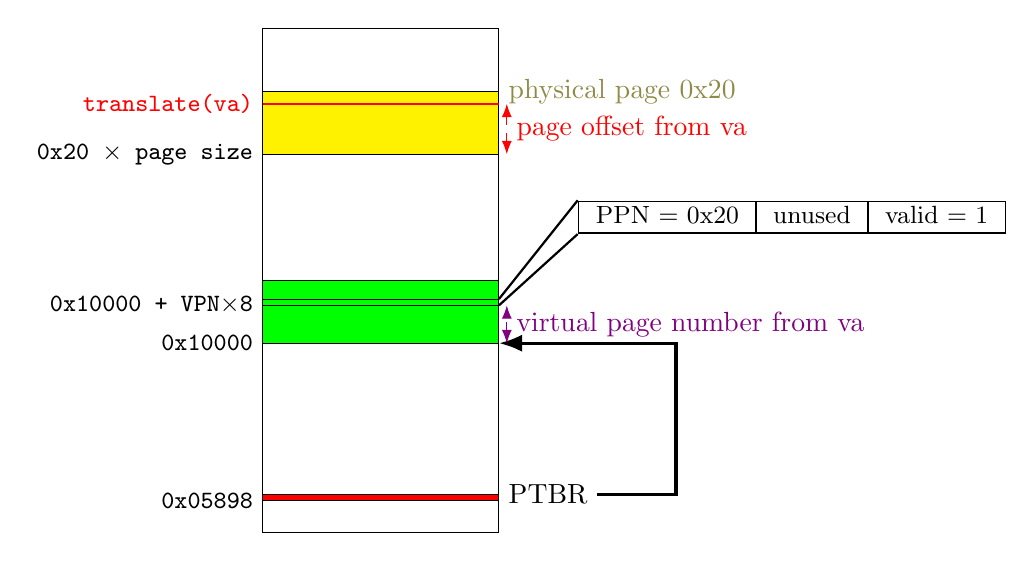
\begin{tikzpicture}
\draw (0, 0) rectangle (3, -8);
\draw[fill=red] (0, -7.5) rectangle (3, -7.4)
    node[right] (ptbr) {PTBR};
\draw[fill=green] (0, -4) rectangle (3, -5);
\draw[-Latex, very thick] (ptbr.east) -- ++(1cm, 0cm) |- (3, -5);
\node[font=\small\tt,anchor=east] at (0, -7.5) {0x05898};
\node[font=\small\tt,anchor=east] at (0, -5) {0x10000};
\node[font=\small\tt,anchor=east] at (0, -4.4) {0x10000 + VPN$\times$8};
\node[font=\small\tt,anchor=east] at (0, -2) {0x20 $\times$ page size};

\draw[Latex-Latex,violet,dashed] (3.1, -5) -- (3.1, -4.4) node[midway,right] {virtual page number from va};
\draw (0, -4.4) rectangle (3, -4.3);
\node[anchor=west,font=\small,inner sep=0mm] (pte) at (4, -3) {
    \begin{tabular}{|l|l|l|} \hline
    PPN = 0x20 & unused & valid = 1 \\ \hline
    \end{tabular}
};
\draw[thick] (3, -4.4) -- (pte.south west);
\draw[thick] (3, -4.3) -- (pte.north west);

\draw[fill=yellow] (0, -2) rectangle (3, -1)
    node[right,yellow!50!black] {physical page 0x20};
\draw[Latex-Latex,red,dashed] (3.1, -2) -- (3.1, -1.2) node[midway, right] {page offset from va};
\draw[thick,red] (0, -1.2) -- (3, -1.2);

\node[red,font=\small\tt,anchor=east] at (0, -1.2) {translate(va)};

\end{tikzpicture}
\end{frame}

\begin{frame}[plain]{first page\_allocate(va) [LEVELS=1]}
\begin{tikzpicture}
\draw (0, 0) rectangle (3, -8);
\draw[fill=red] (0, -7.5) rectangle (3, -7.4)
    node[right] (ptbr) {PTBR};
\begin{visibleenv}<2->
\draw[fill=green] (0, -4) rectangle (3, -5);
\draw[alt=<2>{red},-Latex, very thick] (ptbr.east) -- ++(1cm, 0cm) |- (3, -5);
\end{visibleenv}
\node[font=\small\tt,anchor=east] at (0, -7.5) {0x05898};
\begin{visibleenv}<2->
\node[font=\small\tt,anchor=east] at (0, -5) {NEW0};
\node[font=\small\tt,anchor=east] at (0, -4.4) {NEW0 + VPN$\times$8};

\draw[Latex-Latex,violet,dashed] (3.1, -5) -- (3.1, -4.4) node[midway,right] {virtual page number from va};
\draw (0, -4.4) rectangle (3, -4.3);
\begin{visibleenv}<2>
\node[anchor=west,font=\small,inner sep=0mm] (pte) at (4, -3) {
    \begin{tabular}{|l|l|l|} \hline
    unused & unused & \myemph<2>{valid = 0} \\ \hline
    \end{tabular}
};
\end{visibleenv}
\begin{visibleenv}<3->
\node[draw=red,anchor=west,font=\small,inner sep=0mm] (pte up) at (4, -3) {
    \begin{tabular}{|l|l|l|} \hline
    PPN = \myemph{NEW1} & unused & \myemph<2>{valid = 1} \\ \hline
    \end{tabular}
};
\end{visibleenv}
\draw[thick] (3, -4.4) -- (pte.south west);
\draw[thick] (3, -4.3) -- (pte.north west);

\begin{visibleenv}<3->
\draw[fill=yellow] (0, -2) rectangle (3, -1);
\node[font=\small\tt,anchor=east] at (0, -2) {\myemph{NEW1} $\times$ page size};
\draw[decorate,decoration={brace,mirror}] (3.1, -2) -- (3.1, -1) node[midway,right] {from posix\_memalign};
\end{visibleenv}
\end{tikzpicture}
\end{frame}

\begin{frame}[plain]{page\_allocate(va) [LEVELS=1]}
\begin{tikzpicture}
\draw (0, 0) rectangle (3, -8);
\draw[fill=red] (0, -7.5) rectangle (3, -7.4)
    node[right] (ptbr) {PTBR};
\draw[fill=green] (0, -4) rectangle (3, -5);
\draw[-Latex, very thick] (ptbr.east) -- ++(1cm, 0cm) |- (3, -5);
\node[font=\small\tt,anchor=east] at (0, -7.5) {0x05898};
\node[font=\small\tt,anchor=east] at (0, -5) {0x10000};
\node[font=\small\tt,anchor=east] at (0, -4.4) {0x10000 + VPN$\times$8};

\draw[Latex-Latex,violet,dashed] (3.1, -5) -- (3.1, -4.4) node[midway,right] {virtual page number from va};
\draw (0, -4.4) rectangle (3, -4.3);
\begin{visibleenv}<1>
\node[anchor=west,font=\small,inner sep=0mm] (pte) at (4, -3) {
    \begin{tabular}{|l|l|l|} \hline
    unused & unused & \myemph<2>{valid = 0} \\ \hline
    \end{tabular}
};
\end{visibleenv}
\begin{visibleenv}<2>
\node[draw=red,anchor=west,font=\small,inner sep=0mm] (pte up) at (4, -3) {
    \begin{tabular}{|l|l|l|} \hline
    PPN = \myemph{NEW} & unused & \myemph<2>{valid = 1} \\ \hline
    \end{tabular}
};
\end{visibleenv}
\draw[thick] (3, -4.4) -- (pte.south west);
\draw[thick] (3, -4.3) -- (pte.north west);

\begin{visibleenv}<2->
\draw[fill=yellow] (0, -2) rectangle (3, -1);
\node[font=\small\tt,anchor=east] at (0, -2) {\myemph{NEW} $\times$ page size};
\draw[decorate,decoration={brace,mirror}] (3.1, -2) -- (3.1, -1) node[midway,right] {from posix\_memalign};
\end{visibleenv}

\end{tikzpicture}
\end{frame}


\usetikzlibrary{arrows.meta,fit,matrix}

\begin{frame}{page table lookup (and translate())}
\begin{tikzpicture}
\tikzset{
    >=Latex,
}
\matrix[tight matrix,anchor=north west,
    nodes={text width=2cm,minimum height=0.6cm},
    column 1/.style={nodes={draw=none,font=\tt,align=right}},
    column 2/.style={nodes={draw,thick,font=\tt,text width=1.2cm,align=center}},
    column 3/.style={nodes={draw,thick,font=\tt, text width=3.5cm}},
    column 4/.style={nodes={draw,thick,font=\tt,visible on=<all:0>, text width=1cm}},
    column 5/.style={nodes={draw,thick,font=\tt,visible on=<all:0>, text width=1cm}},
    row 1/.style={nodes={draw=none,font=\normalfont}},
    ] (pt) at (0, 5) {
    virtual page \# \& valid? \& physical page \# \& read OK? \& write OK? \\
    0\ldots0000 \& |[alias=baseAddr]| 1 \& 01000 \& 1 \& 0 \\
    0\ldots0001 \& 1 \& 11111 \& 1 \& 1 \\
    0\ldots0010 \& 0 \& 00000 \& 0 \& 1 \\
    \ldots \& |[draw=none]| \ldots
           \& |[draw=none]| \ldots
           \& |[draw=none]| \ldots
           \& |[draw=none]| \ldots
           \\
    1\ldots1111 \& 0 \& 01100 \& 1 \& 1 \\
};
\node[alt=<2>{red},font=\tt] (ptbr label) at ([xshift=-6cm]baseAddr.north east) {ptbr};
\draw[alt=<2>{red},ultra thick,dotted,->] (ptbr label) -- (baseAddr.north west);
\node[draw,fill=blue!10] (addrLeft) at (-1, 6.0) {\tt 0\ldots0001};
\node[anchor=west,fill=green!10] (addrRest) at (addrLeft.east) {\tt 1101 0010 \normalfont};
\node[anchor=west] (addrDesc) at (addrRest.east) {--- address from CPU (\texttt{\myemph<1>{va}})};
\draw[->,very thick,draw=blue!50!black] (addrLeft.south) |- ([xshift=0ex]pt-3-1.west);
\draw[->,thick] (pt-6-2.south) |- ++(-1cm,-.25cm) -- ++(0cm,-.25cm) node[below,align=center] {trigger exception if 0?\\(\myemph{return \~~0})};
\draw[->,very thick,draw=blue!50!black] ([xshift=3ex]pt-6-3.south west) |- ++(2cm,-.5cm)
    node[right,fill=blue!10] (newAddrLeft) {\tt 111};
\node[anchor=west,fill=green!10] (newAddrRight) at (newAddrLeft.east) {\tt 1101 0010};
\draw[->,very thick,draw=green!50!black] (addrRest) |- ([xshift=1cm,yshift=.5cm]pt-1-3.north east) -| (newAddrRight);
\node[inner sep=0mm,draw=black,thin,fit=(newAddrLeft) (newAddrRight)] (newAddrBox) {};
\draw[->,very thick] (newAddrBox.south) -- ++(0cm,-.5cm) node[below] {to memory (\texttt{\myemph<1>{translate(va)}})};
\end{tikzpicture}
\end{frame}

\begin{frame}{page table lookup (and allocate)}
\begin{tikzpicture}
\tikzset{
    >=Latex,
}
\begin{visibleenv}<2->
\matrix[tight matrix,anchor=north west,
    nodes={text width=2cm,minimum height=0.6cm},
    column 1/.style={nodes={draw=none,font=\tt,align=right}},
    column 2/.style={nodes={draw,thick,font=\tt,text width=1.2cm,align=center}},
    column 3/.style={nodes={draw,thick,font=\tt, text width=3.5cm}},
    column 4/.style={nodes={draw,thick,font=\tt,visible on=<all:0>, text width=1cm}},
    column 5/.style={nodes={draw,thick,font=\tt,visible on=<all:0>, text width=1cm}},
    row 1/.style={nodes={draw=none,font=\normalfont}},
    ] (pt) at (0, 5) {
    virtual page \# \& valid? \& physical page \# \\%\& read OK? \& write OK? \\
    0\ldots0000 \& |[alias=baseAddr]| 1 \& 01000 \\%\& 1 \& 0 \\
    0\ldots0001 \& |[alt=<2>{fill=red!10}]| 0 \& |[alt=<2>{fill=red!10}]| 00000 \\%\& 0 \& 0 \\
    0\ldots0010 \& 0 \& 00000 \& 0 \& 0 \\
    \ldots \& |[draw=none]| \ldots
           \& |[draw=none]| \ldots
           \\ %\& |[draw=none]| \ldots \& |[draw=none]| \ldots \\
    1\ldots1111 \& 0 \& 01100 \\ %\& 1 \& 1 \\
};
\end{visibleenv}
\node[alt=<1>{red},font=\tt] (ptbr label) at ([xshift=-6cm]baseAddr.north east) {ptbr};
\draw[alt=<1>{red},ultra thick,dotted,->] (ptbr label) -- (baseAddr.north west);
\begin{visibleenv}<1>
\node[draw=red,ultra thick] at (pt) {
    page\_allocate(va) --- set ptbr if unset
};
\end{visibleenv}
\node[draw,fill=blue!10] (addrLeft) at (-1, 6.0) {\tt 0\ldots0001};
\node[anchor=west,fill=green!10] (addrRest) at (addrLeft.east) {\tt 1101 0010 \normalfont};
\node[anchor=west] (addrDesc) at (addrRest.east) {--- address from CPU (\texttt{\myemph<1>{va}})};
    \draw[->,very thick,draw=blue!50!black] (addrLeft.south) |- ([xshift=0ex]pt-3-1.west);
    \draw[->,thick] (pt-6-2.south) |- ++(-1cm,-.25cm) -- ++(0cm,-.25cm) node[below,align=center] {trigger exception if 0?\\(\myemph{return \~~0})};
\draw[->,very thick,draw=blue!50!black] ([xshift=3ex]pt-6-3.south west) |- ++(2cm,-.5cm)
    node[right,fill=blue!10] (newAddrLeft) {\tt 111};
    \node[anchor=west,fill=green!10] (newAddrRight) at (newAddrLeft.east) {\tt 1101 0010};
\draw[->,very thick,draw=green!50!black] (addrRest) |- ([xshift=1cm,yshift=.5cm]pt-1-3.north east) -| (newAddrRight);
    \node[inner sep=0mm,draw=black,thin,fit=(newAddrLeft) (newAddrRight)] (newAddrBox) {};
    \draw[->,very thick] (newAddrBox.south) -- ++(0cm,-.5cm) node[below] {to memory (\texttt{\myemph<1>{translate(va)}})};
\begin{visibleenv}<2>
\node[align=left,draw=red,ultra thick,anchor=west] at ([xshift=-2cm]pt.east) {
    page\_allocate(va) --- \\set page table entry \\ if unset
};
\end{visibleenv}
\end{tikzpicture}
\end{frame}


\section{handling big page tables}
\subsection{the problem}
\usetikzlibrary{positioning,shapes.callouts}

\begin{frame}[fragile,label=64bExA]{exercise: 64-bit system}
\begin{itemize}
\item my desktop: 39-bit physical addresses; \myemph<2>{48-bit\tikzmark{virtAddr} virtual addresses}
\item 4096 byte pages
\item<3-> exercise: how many page table entries? (assuming page table like shown before)
    \only<4->{\iftoggle{heldback}{}{$2^{48} / 2^{12} = 2^{36}$ entries}}
\item<3-> exercise: how large are physical page numbers?
    \only<4->{\iftoggle{heldback}{}{$39 - 12 = 27$ bits}}
\item<5-> page table entries are \myemph{8 bytes} (room for expansion, metadata)
    \begin{itemize}
    \item trick: power of two size makes table lookup faster
    \end{itemize}
\item<5-> would take up $2^{39}$ bytes?? (512GB??)
\end{itemize}
\begin{tikzpicture}[overlay,remember picture]
\begin{visibleenv}<2>
\node[my callout=virtAddr,align=center] at ([yshift=-1cm,xshift=-8cm]pic cs:virtAddr) {
    top 16 bits of 64-bit addresses not used for translation
};
\end{visibleenv}
\end{tikzpicture}
\end{frame}


\subsection{general options}
\usetikzlibrary{patterns,positioning,calc,fit}

\begin{frame}{huge page tables}
\begin{itemize}
    \item huge virtual address spaces!
    \item impossible to store PTE for every page
    \vspace{.5cm}
    \item how can we save space?
\end{itemize}
\end{frame}

\begin{frame}{holes}
\begin{tikzpicture}
\tikzset{
    mylabel/.style={font=\ttfamily},
    mybox/.style={draw,rectangle,minimum width=7cm,fill=white,inner sep=1mm},
    myhigh/.style={draw,rectangle,line width=1mm, draw=blue!80!black,opacity=.3},
}
\begin{scope}[name prefix=A-]
\node[mybox,minimum height=1cm,pattern=north west lines,pattern color=black!5!white] (kernel) {Used by OS};
\node[mybox, minimum height=.5cm, below=1cm of kernel] (stack) {Stack};
\node[mybox, minimum height=.5cm, below=1cm of stack] (heap) {Heap / other dynamic};
\node[mybox, minimum height=.5cm, below=0mm of heap] (data) {Writable data};
\node[mybox, minimum height=.5cm, below=0mm of data] (sdata) {Code + Constants};
\coordinate (memBottom) at ($(sdata.south east) + (0mm, -2mm)$);
\begin{pgfonlayer}{bg}
\draw[pattern=north west lines, pattern color=black!40!white] (kernel.north west) rectangle (memBottom);
\end{pgfonlayer}
\node[fill=red,fill opacity=0.05,inner sep=0mm,draw=red,ultra thick,fit=(kernel.south west) (stack.north east)] {};
\node[fill=red,fill opacity=0.05,inner sep=0mm,draw=red,ultra thick,fit=(stack.south west) (heap.north east)] {};
\node[fill=red,fill opacity=0.05,inner sep=0mm,draw=red,ultra thick,fit=(sdata.south west) (memBottom)] {};
\end{scope}
\node[right=1cm of A-stack] {most pages are \myemph{invalid}};
\end{tikzpicture}
\end{frame}

\begin{frame}{saving space}
\begin{itemize}
    \item basic idea: don't store (most) invalid page table entries
    \item use a data structure other than a flat array
        \begin{itemize}
        \item want a map --- lookup key (virtual page number), get value (PTE)
        \end{itemize}
    \item options?
    \vspace{.5cm}
    \item<2-> \myemph<2>{hashtable}
        \begin{itemize}
        \item<2-> actually used by some historical processors
        \item<2-> but never common
        \end{itemize}
    \item<3-> \myemph<3>{tree data structure}
        \begin{itemize}
        \item<3-> but not quite a search tree
        \end{itemize}
\end{itemize}
\end{frame}

\begin{frame}{search tree tradeoffs}
    \begin{itemize}
    \item lookup usually implemented \myemph{in hardware}
        \begin{itemize}
        \item lookup should be simple
        \item solution: lookup splits up address bits (no complex calculations)
        \end{itemize}
    \item lookup should not involve many memory accesses
        \begin{itemize}
        \item doing two memory accesses is already very slow
        \item solution: tree with many children from each node
            \begin{itemize}
            \item (far from binary tree's left/right child)
            \end{itemize}
        \end{itemize}
    \end{itemize}
\end{frame}



\subsection{two-level page tables}
\usetikzlibrary{arrows.meta, fit}
\begin{frame}<0>[label=twoLevelPtLookup]{two-level page table lookup}
\begin{tikzpicture}
\tikzset{
    >=Latex,
    pageNumber/.style={fill=blue!10,font=\fontsize{11}{12}\selectfont,inner sep=.5mm},
    pageNumberA/.style={fill=violet!30,font=\fontsize{11}{12}\selectfont,inner sep=.5mm,draw,thick,dotted},
    pageNumberB/.style={fill=brown!20,font=\fontsize{11}{12}\selectfont,inner sep=.5mm,draw,thick,dotted},
    pageOffset/.style={fill=green!20,font=\fontsize{11}{12}\selectfont,inner sep=.5mm},
    comp/.style={fill=yellow!10,font=\fontsize{11}{12}\selectfont,draw},
    memAccess/.style={alt=<all:7>{red, very thick}},
    pageNumberExpand/.style={alt=<all:11>{draw=red,very thick}},
    smallLabel/.style={fill=white,draw,thick,font=\fontsize{10}{11}\selectfont,inner sep=.5mm,align=center},
}
\node[pageNumberA] (addrLeftA) {11 0101 01};
\node[pageNumberB,anchor=west] (addrLeftB) at (addrLeftA.east) {00 1011 00};
\node[anchor=west,pageOffset] (addrRight) at (addrLeftB.east) {00 1101 1111};
\node[inner sep=0mm,draw=none,fit=(addrLeftA) (addrLeftB),alt=<1>{draw=red,very thick}] (addrLeft) {};
\begin{visibleenv}<all:1>
\node[below=1cm of addrLeft,xshift=2cm] (vpn split explain) {VPN --- split into two parts (one per level)};
\node[below=1cm of vpn split explain,font=\small] {
    this example: parts equal sized --- common, but not required
};
\end{visibleenv}
\begin{visibleenv}<all:2->
\node[draw,comp,below=1cm of addrLeftA,align=center,xshift=-1cm] (timesPte) {$\times$ \\ PTE \\ size};
\draw[->,thick] (addrLeftA) -- ++(0cm,-.5cm) -| (timesPte);
\node[font=\tt\fontsize{10}{11}\selectfont,draw,very thick,left=0.25cm of addrLeft,label={[align=center,font=\small]north:page table\\base register},yshift=-.5cm] (ptbr) {0x10000};
\node[draw,comp] (plus) at ([yshift=-1cm]timesPte.south) {+};
\draw[->,thick] (timesPte) -- (plus);
\draw[->,thick] (ptbr) |- (plus);
\end{visibleenv}

\begin{visibleenv}<all:3->
\node[below=1.5cm of plus,fill=violet!10,draw,very thick,minimum height=1cm,minimum width=15cm,xshift=5.5cm] (cache) {memory {\small (really cache)}};
\end{visibleenv}
\begin{visibleenv}<all:5->
\node[pageNumber] (addrLeftFinal) at ([xshift=9.6cm,yshift=-1cm]plus) {1101 0011 11};
\end{visibleenv}
\begin{visibleenv}<all:3->
\draw[->,thick,memAccess] (plus) -- (cache.north -| plus.south) node[midway,smallLabel] {1st PTE \\ addr.};
\node[above right=1cm and .5cm of plus,align=center,draw,comp,font=\small] (check) {valid, etc?};
\node[below=.75cm of check,draw,comp,align=center] (splitA) {split  \\ PTE parts};
\draw[->,thick] (cache.north -| splitA.south) -- (splitA.south);
\draw[->,thick] (splitA) -- (check);
\draw[->,thick] (check.north) -- ++(0,.75cm) node[above,font=\small,inner sep=.5mm] {cause fault?};
\end{visibleenv}

\begin{visibleenv}<all:4->
    \node[comp,align=center,right=.75cm of splitA,pageNumberExpand] (timesSize){$\times$ \\ page \\ size};
    \node[comp,align=center,right=1.25cm of timesSize] (plusB) {+};
    \draw[brown!60!black,->,thick,pageNumberExpand] (splitA) -- (timesSize);
    \draw[dotted,black,thick] ($(splitA.east)!0.5!(timesSize.west)$) -- ++ (0cm, .5cm) node[above,font=\fontsize{10}{11}\selectfont,align=center] {phys\\page \#};
    \draw[brown!60!black,->,thick,pageNumberExpand] (timesSize) -- (plusB);
    \draw[dotted,black,thick] ($(plusB.east)!0.5!(timesSize.west)$) -- ++ (0cm, .5cm) node[above,font=\fontsize{10}{11}\selectfont,align=center] {phys\\addr};
    \draw[memAccess,->,thick] (plusB) -- (plusB |- cache.north) node[midway,smallLabel]{2nd PTE \\ addr.};
    \node[comp,align=center,above=.5cm of plusB] (timesPteB) {$\times$ \\ PTE \\ size};
    \draw[brown!60!black,->,thick] (addrLeftB) -- ++(0cm,-.5cm) -| (timesPteB.north);
    \draw[brown!60!black,->,thick] (timesPteB) -- (plusB);
\end{visibleenv}

\begin{visibleenv}<all:5->
\node[right=.5cm of plusB,draw,comp,align=center] (splitB) {split  \\ PTE parts};
\draw[->,thick] (cache.north -| splitB.south) -- (splitB.south);
\node[above=.75cm of splitB,align=center,draw,comp,font=\small] (checkB) {valid, etc?};
\draw[->,thick] (splitB) -- (checkB);
\draw[->,thick] (checkB.north) -- ++(0cm, .75cm) node[above,font=\small,inner sep=.5mm] {cause fault?};
\draw[blue!50!black,->,thick] (splitB) -| (addrLeftFinal);
\end{visibleenv}

\begin{visibleenv}<all:6->
\node[anchor=west,pageOffset] (addrRightFinal) at (addrLeftFinal.east) {00 1101 1111};
%\draw[very thick,green!50!black,densely dotted] (addrRight) |- ([xshift=-.5mm,yshift=.5cm]splitA.north);
\draw[very thick,green!50!black,densely dotted,->] (addrRight) -| (addrRightFinal.north);
\end{visibleenv}
\begin{visibleenv}<all:3->
\node[inner sep=0mm,draw,label={[font=\fontsize{12}{13}\selectfont]south:physical address},fit=(addrLeftFinal) (addrRightFinal)] (addrFinal) {};
\end{visibleenv}

\node[inner sep=0mm,draw,label={[font=\fontsize{12}{13}\selectfont]north:virtual address},fit=(addrLeft) (addrRight)] (addr) {};
\begin{visibleenv}<all:5->
    \draw[->,thick,memAccess] (addrFinal) -- (cache.north -| addrFinal.south);
\end{visibleenv}

\begin{pgfonlayer}{bg}
\begin{visibleenv}<all:8,10>
    \node [fill=violet!5,fit=(timesPte) (splitA),draw,line width=0.125mm,dashed] (firstBox) {};
\end{visibleenv}
\begin{visibleenv}<all:9,10>
    \node [fill=brown!5,fit=(timesPteB) (splitB),draw,line width=0.125mm,dashed] (secondBox) {};
\end{visibleenv}

\begin{visibleenv}<all:12>
    \node [fill=black!5,fit=(timesPte) (splitA) (timesPteB) (splitB),draw,line width=0.5mm,dashed,label={south:MMU}] (mmu) {};
\end{visibleenv}
\end{pgfonlayer}
 
\begin{visibleenv}<all:8> 
\node [fill=white,fill opacity=0.9,anchor=north] at (firstBox.south) {first-level page table lookup};
\end{visibleenv}

\begin{visibleenv}<all:9> 
\node [fill=white,fill opacity=0.9,anchor=north] at (secondBox.south) {second-level page table lookup};
\end{visibleenv}
 
\begin{visibleenv}<all:10> 
\node [fill=white,fill opacity=0.9,anchor=north] at (firstBox.south) {first-level};
\end{visibleenv}

\begin{visibleenv}<all:10> 
\node [fill=white,fill opacity=0.9,anchor=north] at (secondBox.south) {second-level};
\end{visibleenv}

\begin{visibleenv}<all:11>
\node[fill=white,fill opacity=0.9,anchor=south,align=center] at (timesSize.north) {
    have physical page number \\
    need address of first byte of page 
};
\end{visibleenv}
\end{tikzpicture}
\end{frame}

\usetikzlibrary{arrows.meta,matrix,shapes.misc,calc,fit,positioning}

% FIXME: with VPN ranges labelled?
\begin{frame}<all:1-8>[fragile,label=twoLevelPT]{two-level page tables}
\begin{tikzpicture}
\tikzset{
    >=Latex,
    ptr/.style={->,very thick},
    ptNode/.style={minimum height=.5cm,text width=4.5cm,thick},
    ptNodeW/.style={minimum height=.5cm,text width=5.5cm,thick},
    firstLevel/.style={blue!40!black},
    secondLevel/.style={green!40!black},
}
\matrix[tight matrix,firstLevel,
    nodes={ptNodeW},
    label={north:first-level page table},
    ] (first) {
        for VPN 0x0-0xFF  \\
        for VPN 0x100-0x1FF \\
        for VPN 0x200-0x2FF \\
        for VPN 0x300-0x300 \\
        |[draw=none,align=center]| \ldots \\
        for VPN 0xFF00-0xFFFF \\
    };
\node[anchor=north west] at ([yshift=3.5cm]first.north west) {
two-level page tables for 65536 pages (16-bit VPN; 256 entries/table)
};
\matrix[tight matrix,anchor=north west,secondLevel,
nodes={ptNode},
label={north:second-level page tables},
] (secondOne) at ([xshift=1cm,yshift=2cm]first.north east) {
    PTE for VPN 0x00 \\
    PTE for VPN 0x01 \\
    PTE for VPN 0x02 \\
    PTE for VPN 0x03 \\
    |[draw=none,align=center]| \ldots \\
    PTE for VPN 0xFF \\
};
\draw[ptr] ([xshift=-.5cm]first-1-1.east) [fill] circle (1mm);
\draw[ptr] ([xshift=-.5cm]first-1-1.east) -- (secondOne-1-1.west);
\draw[ptr] ([xshift=-.5cm]secondOne-1-1.east) [fill] circle (1mm);
\draw[ptr] ([xshift=-.5cm]secondOne-1-1.east) -- ++(1cm,0cm) node[right,align=left] {actual data for page \\ (if PTE valid)};
\matrix[tight matrix,anchor=north west,secondLevel,
nodes={ptNode},
] (secondTwo) at ([xshift=1.5cm,yshift=-1.5cm]first.north east) {
    PTE for VPN 0x300 \\
    PTE for VPN 0x301 \\
    PTE for VPN 0x302\\
    PTE for VPN 0x303 \\
    |[draw=none,align=center]| \ldots \\
    PTE for VPN 0x3FF \\
};
\draw[ptr] ([xshift=-.5cm]first-4-1.east) [fill] circle (1mm);
\draw[ptr] ([xshift=-.5cm]first-4-1.east) -- (secondTwo-1-1.west);
\begin{visibleenv}<all:2->
\foreach \x in {2,3} {
\draw[thick,red] ([xshift=-.5cm]first-\x-1.east) node[draw=red,cross out,minimum width=.25cm,minimum height=.25cm] {};
}
\end{visibleenv}
\begin{visibleenv}<all:2>
    \node[draw=red,ultra thick,inner sep=0mm,fit=(first-2-1) (first-3-1),label={[draw=red,ultra thick,label distance=2mm,fill=white]east:invalid entries represent big holes}] {};
\end{visibleenv}
\begin{pgfonlayer}{fg}
\begin{visibleenv}<all:3-5>
\matrix[tight matrix,anchor=north west,firstLevel,
    nodes={minimum height=.55cm},
    label={[alias=firstZoomLabel,font=\bfseries]north:first-level page table},
    column 1/.style={nodes={draw=none,font=\tt,text width=4cm}},
    column 2/.style={nodes={text width=1.3cm,font=\tt,align=center}},
    column 3/.style={nodes={text width=1.3cm,font=\tt,align=center}},
    column 4/.style={nodes={text width=3.6cm,font=\tt,align=left,
        alt=<all:4>{red}}},
    row 1/.style={nodes={font=\normalfont,draw=none,black}},
] (firstZoom) at ([xshift=-2cm,yshift=2cm]first.north east) {
    VPN range \& valid \& \ldots \& physical page \# \small (of \myemph<all:4>{next page table}) \\
    0x\myemph<all:5>{00}00-0x\myemph<all:5>{00}FF \& 1 \& \ldots \& 0x22343 \\
    0x\myemph<all:5>{01}00-0x\myemph<all:5>{01}FF \& 0 \& \ldots \& 0x00000 \\
    0x\myemph<all:5>{02}00-0x\myemph<all:5>{02}FF \& 0 \& \ldots \& 0x00000 \\
    0x\myemph<all:5>{03}00-0x\myemph<all:5>{03}FF \& 1 \& \ldots \& 0x33454 \\
    0x\myemph<all:5>{04}00-0x\myemph<all:5>{04}FF \& 1 \& \ldots \& 0xFF043 \\
    \ldots \& \ldots \& \ldots \& \ldots \& \ldots \\
    0x\myemph<all:5>{FF}00-0x\myemph<all:5>{FF}FF \& 1 \& \ldots \& 0xFF045 \\
} ;
\end{visibleenv}

\begin{visibleenv}<all:6-7>
\matrix[tight matrix,anchor=north west,secondLevel,
    nodes={minimum height=.55cm},
    label={[alias=secondZoomLabel,font=\bfseries]north:a second-level page table},
    column 1/.style={nodes={draw=none,font=\tt,text width=1.7cm}},
    column 2/.style={nodes={text width=1.3cm,font=\tt,align=center}},
    column 3/.style={nodes={text width=1.3cm,font=\tt,align=center}},
    column 4/.style={nodes={text width=3.6cm,font=\tt,align=left,
        alt=<all:4>{red}}},
    row 1/.style={nodes={font=\normalfont,draw=none,black}},
] (secondZoom) at ([xshift=.5cm,yshift=2cm]first.north east) {
    VPN \& valid \& \ldots \& physical page \# \small (of data) \\
    0x3\myemph<all:7>{00} \& 0 \& 1 \& 0x42443 \\
    0x3\myemph<all:7>{01} \& 0 \& 1 \& 0x4A9DE \\
    0x3\myemph<all:7>{02} \& 0 \& 1 \& 0x5C001 \\
    0x3\myemph<all:7>{03} \& 0 \& 1 \& 0x00000 \\
    0x3\myemph<all:7>{04} \& 0 \& 1 \& 0x6C223 \\
    \ldots \& \ldots \& \ldots \& \ldots \\
    0x3\myemph<all:7>{FF} \& \ldots \& 1 \& 0x00000 \\
} ;
\end{visibleenv}
\end{pgfonlayer}

\begin{visibleenv}<all:3-5>
\node[draw,fit=(firstZoom) (firstZoomLabel),fill=white] (firstZoomBox) {};
    \draw[ultra thick,dotted] (first.north west) -- (firstZoomBox.north west);
    \draw[ultra thick,dotted] (first-6-1.south west) -- (firstZoomBox.south west);
    %\draw[ultra thick,dotted] (first-4-1.south east) -- (firstZoomBox.south east);
\end{visibleenv}

\begin{visibleenv}<all:6-7>
\node[draw,fit=(secondZoom) (secondZoomLabel),fill=white] (secondZoomBox) {};
    %\draw[ultra thick,dotted] (secondTwo.north west) -- (secondZoomBox.north west);
    %\draw[ultra thick,dotted] (secondTwo.north east) -- (secondZoomBox.north east);
    \draw[ultra thick,dotted] (secondTwo.south west) -- (secondZoomBox.south west);
    \draw[ultra thick,dotted] (secondTwo.south east) -- (secondZoomBox.south east);
\end{visibleenv}


% FIXME: color code for each page table
\end{tikzpicture}
\end{frame}

\begin{frame}{two-level page table lookup}
\begin{tikzpicture}
\tikzset{
    >=Latex,
    pageNumber/.style={fill=blue!10,font=\fontsize{11}{12}\selectfont,inner sep=.5mm},
    pageNumberA/.style={fill=violet!20,font=\fontsize{11}{12}\selectfont,inner sep=.5mm},
    pageNumberB/.style={fill=brown!20,font=\fontsize{11}{12}\selectfont,inner sep=.5mm},
    pageOffset/.style={fill=green!20,font=\fontsize{11}{12}\selectfont,inner sep=.5mm},
    comp/.style={fill=yellow!10,font=\fontsize{11}{12}\selectfont,draw},
    memAccess/.style={alt=<all:7>{red, very thick}},
    pageNumberExpand/.style={alt=<all:11>{draw=red,very thick}},
    smallLabel/.style={fill=white,draw,thick,font=\fontsize{10}{11}\selectfont,inner sep=.5mm,align=center},
}
\node[pageNumberA] (addrLeftA) {11 0101 01};
\node[pageNumberB,anchor=west] (addrLeftB) at (addrLeftA.east) {00 1011 00};
\node[anchor=west,pageOffset] (addrRight) at (addrLeftB.east) {00 1101 1111};
\node[inner sep=0mm,draw=none,fit=(addrLeftA) (addrLeftB),alt=<1>{draw=red,very thick}] (addrLeft) {};
\begin{visibleenv}<all:1>
\node[below=1cm of addrLeft,xshift=2cm] (vpn split explain) {VPN --- split into two parts (one per level)};
\node[below=1cm of vpn split explain,font=\small] {
    this example: parts equal sized --- common, but not required
};
\end{visibleenv}
\begin{visibleenv}<all:2->
\node[draw,comp,below=1cm of addrLeftA,align=center,xshift=-1cm] (timesPte) {$\times$ \\ PTE \\ size};
\draw[->,thick] (addrLeftA) -- ++(0cm,-.5cm) -| (timesPte);
\node[font=\tt\fontsize{10}{11}\selectfont,draw,very thick,left=0.25cm of addrLeft,label={[align=center,font=\small]north:page table\\base register},yshift=-.5cm] (ptbr) {0x10000};
\node[draw,comp] (plus) at ([yshift=-1cm]timesPte.south) {+};
\draw[->,thick] (timesPte) -- (plus);
\draw[->,thick] (ptbr) |- (plus);
\end{visibleenv}

\begin{visibleenv}<all:3->
\node[below=1.5cm of plus,fill=violet!10,draw,very thick,minimum height=1cm,minimum width=15cm,xshift=5.5cm] (cache) {memory {\small (really cache)}};
\end{visibleenv}
\begin{visibleenv}<all:5->
\node[pageNumber] (addrLeftFinal) at ([xshift=9.6cm,yshift=-1cm]plus) {1101 0011 11};
\end{visibleenv}
\begin{visibleenv}<all:3->
\draw[->,thick,memAccess] (plus) -- (cache.north -| plus.south) node[midway,smallLabel] {1st PTE \\ addr.};
\node[above right=1cm and .5cm of plus,align=center,draw,comp,font=\small] (check) {valid, etc?};
\node[below=.75cm of check,draw,comp,align=center] (splitA) {split  \\ PTE parts};
\draw[->,thick] (cache.north -| splitA.south) -- (splitA.south);
\draw[->,thick] (splitA) -- (check);
\draw[->,thick] (check.north) -- ++(0,.75cm) node[above,font=\small,inner sep=.5mm] {cause fault?};
\end{visibleenv}

\begin{visibleenv}<all:4->
    \node[comp,align=center,right=.75cm of splitA,pageNumberExpand] (timesSize){$\times$ \\ page \\ size};
    \node[comp,align=center,right=1.25cm of timesSize] (plusB) {+};
    \draw[brown!60!black,->,thick,pageNumberExpand] (splitA) -- (timesSize);
    \draw[dotted,black,thick] ($(splitA.east)!0.5!(timesSize.west)$) -- ++ (0cm, .5cm) node[above,font=\fontsize{10}{11}\selectfont,align=center] {phys\\page \#};
    \draw[brown!60!black,->,thick,pageNumberExpand] (timesSize) -- (plusB);
    \draw[dotted,black,thick] ($(plusB.east)!0.5!(timesSize.west)$) -- ++ (0cm, .5cm) node[above,font=\fontsize{10}{11}\selectfont,align=center] {phys\\addr};
    \draw[memAccess,->,thick] (plusB) -- (plusB |- cache.north) node[midway,smallLabel]{2nd PTE \\ addr.};
    \node[comp,align=center,above=.5cm of plusB] (timesPteB) {$\times$ \\ PTE \\ size};
    \draw[brown!60!black,->,thick] (addrLeftB) -- ++(0cm,-.5cm) -| (timesPteB.north);
    \draw[brown!60!black,->,thick] (timesPteB) -- (plusB);
\end{visibleenv}

\begin{visibleenv}<all:5->
\node[right=.5cm of plusB,draw,comp,align=center] (splitB) {split  \\ PTE parts};
\draw[->,thick] (cache.north -| splitB.south) -- (splitB.south);
\node[above=.75cm of splitB,align=center,draw,comp,font=\small] (checkB) {valid, etc?};
\draw[->,thick] (splitB) -- (checkB);
\draw[->,thick] (checkB.north) -- ++(0cm, .75cm) node[above,font=\small,inner sep=.5mm] {cause fault?};
\draw[blue!50!black,->,thick] (splitB) -| (addrLeftFinal);
\end{visibleenv}

\begin{visibleenv}<all:6->
\node[anchor=west,pageOffset] (addrRightFinal) at (addrLeftFinal.east) {00 1101 1111};
%\draw[very thick,green!50!black,densely dotted] (addrRight) |- ([xshift=-.5mm,yshift=.5cm]splitA.north);
\draw[very thick,green!50!black,densely dotted,->] (addrRight) -| (addrRightFinal.north);
\end{visibleenv}
\begin{visibleenv}<all:3->
\node[inner sep=0mm,draw,label={[font=\fontsize{12}{13}\selectfont]south:physical address},fit=(addrLeftFinal) (addrRightFinal)] (addrFinal) {};
\end{visibleenv}

\node[inner sep=0mm,draw,label={[font=\fontsize{12}{13}\selectfont]north:virtual address},fit=(addrLeft) (addrRight)] (addr) {};
\begin{visibleenv}<all:5->
    \draw[->,thick,memAccess] (addrFinal) -- (cache.north -| addrFinal.south);
\end{visibleenv}

\begin{pgfonlayer}{bg}
\begin{visibleenv}<all:8,10>
    \node [fill=violet!5,fit=(timesPte) (splitA),draw,line width=0.125mm,dashed] (firstBox) {};
\end{visibleenv}
\begin{visibleenv}<all:9,10>
    \node [fill=brown!5,fit=(timesPteB) (splitB),draw,line width=0.125mm,dashed] (secondBox) {};
\end{visibleenv}

\begin{visibleenv}<all:12>
    \node [fill=black!5,fit=(timesPte) (splitA) (timesPteB) (splitB),draw,line width=0.5mm,dashed,label={south:MMU}] (mmu) {};
\end{visibleenv}
\end{pgfonlayer}
 
\begin{visibleenv}<all:8> 
\node [fill=white,fill opacity=0.9,anchor=north] at (firstBox.south) {first-level page table lookup};
\end{visibleenv}

\begin{visibleenv}<all:9> 
\node [fill=white,fill opacity=0.9,anchor=north] at (secondBox.south) {second-level page table lookup};
\end{visibleenv}
 
\begin{visibleenv}<all:10> 
\node [fill=white,fill opacity=0.9,anchor=north] at (firstBox.south) {first-level};
\end{visibleenv}

\begin{visibleenv}<all:10> 
\node [fill=white,fill opacity=0.9,anchor=north] at (secondBox.south) {second-level};
\end{visibleenv}

\begin{visibleenv}<all:11>
\node[fill=white,fill opacity=0.9,anchor=south,align=center] at (timesSize.north) {
    have physical page number \\
    need address of first byte of page 
};
\end{visibleenv}
\end{tikzpicture}
\end{frame}

\usetikzlibrary{arrows.meta}
\begin{frame}{another view}
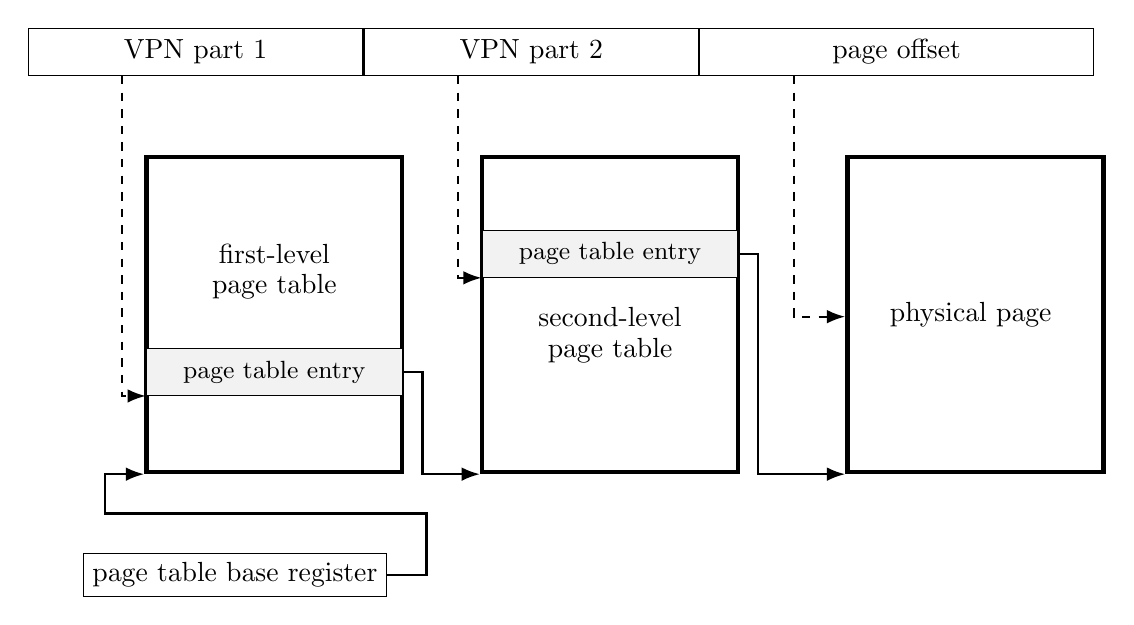
\begin{tikzpicture}
    \tikzset{
        addrPart/.style={draw,minimum height=.6cm},
        pt/.style={draw,ultra thick,minimum height=4cm,minimum width=3.25cm,align=center},
        pte/.style={draw,thin,minimum height=.6cm,minimum width=3.25cm,font=\small,fill=black!5},
        >=Latex,
        compute/.style={thick,->},
        computeB/.style={thick,->,dashed},
    }
    \node[addrPart,minimum width=4.25cm] (vpn1) {VPN part 1};
    \node[addrPart,right=0cm of vpn1,minimum width=4.25cm] (vpn2) {VPN part 2};
    \node[addrPart,right=0cm of vpn2,minimum width=5cm] (po) {page offset};

    \node[pt,below=1cm of vpn1,xshift=1cm] (first) {
        first-level \\
        page table \\
        ~ \\
        ~ \\
    };
    
    \node[draw,below=1cm of first,xshift=-.5cm] (ptbr) {page table base register};
    \draw[compute] (ptbr.east) -- ++(.5cm,0cm) |- ([xshift=-.5cm,yshift=-.5cm]first.south west) |- (first.south west);
    \node[pte] (pte1) at ([yshift=1.3cm]first.south) {page table entry};
    \draw[computeB] ([xshift=1.2cm]vpn1.south west) |- (pte1.south west);

    \node[pt,below=1cm of vpn2,xshift=1cm] (second) {
        ~ \\
        ~ \\
        second-level \\
        page table
    };
    
    \draw[compute] (pte1.east) -- ++(.25cm,0cm) |- (second.south west);
    
    \node[pte] (pte2) at ([yshift=2.8cm]second.south) {page table entry};
    \draw[computeB] ([xshift=1.2cm]vpn2.south west) |- (pte2.south west);
    
    \node[pt,below=1cm of po,xshift=1cm] (final) {
        physical page
    };
    \draw[compute] (pte2.east) -- ++(.25cm,0cm) |- (final.south west);
    \draw[computeB] ([xshift=1.2cm]po.south west) |- ([yshift=2cm]final.south west);
\end{tikzpicture}
\end{frame}


\subsection{more than two levels}
\begin{frame}{multi-level page tables}
    \begin{itemize}
    \item VPN split into pieces for each level of page table
    \vspace{.5cm}
    \item top levels: page table entries point to next page table
        \begin{itemize}
        \item usually using physical page number of next page table
        \end{itemize}
    \item bottom level: page table entry points to destination page
    \vspace{.5cm}
    \item validity checks at \myemph{each level}
    \end{itemize}
\end{frame}

\begin{frame}{x86-64 page table splitting}
    \begin{itemize}
    \item 48-bit virtual address
    \item 12-bit page offset (4KB pages)
    \item 36-bit virtual page number, split into four 9-bit parts
    \item page tables at each level: $2^9$ entries, 8 bytes/entry
        \begin{itemize}
        \item deliberate choice: each page table is one page
        \end{itemize}
    \end{itemize}
\end{frame}

\begin{frame}{note on VPN splitting}
    \begin{itemize}
    \item textbook labels it `VPN 1' and `VPN 2' and so on
    \item these are \myemph{parts of the virtual page number}
        \begin{itemize}
        \item (there are not multiple VPNs)
        \end{itemize}
    \end{itemize}
\end{frame}


\subsection{assignment preview}
% FIXME:assignment preview slides
\begin{frame}{assignment}
\end{frame}

\subsection{exercises: multi-level lookup}
% FIXME: \subsubsection{part 0}
% FIXME: \begin{frame}{splitting addresses for levels}
\begin{itemize}
\item x86-32
\item 32-bit physical address; 32-bit virtual address
\item $2^{12}$ byte page size 
\begin{itemize}\item<2->\iftoggle{heldback}{}{\textit{12-bit page offset}}\end{itemize}
\item 2-levels of page tables; each page table is one page
\item 4 byte page table entries
\begin{itemize}\item<3->\iftoggle{heldback}{}{\textit{$2^{12}/4 = 2^{10}$ PTEs/page table; 10-bit VPN parts}}\end{itemize}
\vspace{.5cm}
\item how is address {\tt 0x12345678} split up?
\begin{itemize}
\item \iftoggle{heldback}{}{\only<4->{10-bit VPN part 1: {\tt 0001 0010 00 (0x48)}; \\ 10-bit VPN part 2: {\tt 11 0100 0101 (0x345)}; \\ 12-bit page offset: {\tt 0x678}}}
\end{itemize}
\end{itemize}
\end{frame}



\subsubsection{part 2}
\usetikzlibrary{matrix,positioning}

\begin{frame}{2-level example}
\begin{itemize}
\item {}\myemph<1>{9-bit} virtual addresses, 6-bit physical; 8 byte pages, 1 byte PTE
\item page tables 1 page; PTE: 3 bit PPN (MSB), 1 valid bit, 4 unused
\item page table base register {\tt 0x20}; translate virtual address {\tt 0x131}
\end{itemize}
\begin{tikzpicture}
\matrix[tight matrix,anchor=north west,
    nodes={text width=2cm,minimum height=0.5cm,font=\small},
    column 1/.style={nodes={draw=none,font=\small\tt,align=right}},
    column 2/.style={nodes={draw,thick,font=\small\tt,text width=2.6cm,align=left}},
    row 1/.style={nodes={draw=none,font=\small\normalfont}},
    ] (memA)  {
    physical addresses \& bytes \\
    0x00-3 \& 00 11 22 33 \\
    0x04-7 \& 44 55 66 77 \\
    0x08-B \& 88 99 AA BB \\
    0x0C-F \& CC DD EE FF \\
    0x10-3 \& 1A 2A 3A 4A \\
    0x14-7 \& 1B 2B 3B 4B \\
    0x18-B \& 1C 2C 3C 4C \\
    0x1C-F \& 1C 2C 3C 4C \\
};
\matrix[tight matrix,anchor=north west,
    nodes={text width=2cm,minimum height=0.5cm,font=\small},
    column 1/.style={nodes={draw=none,font=\small\tt,align=right}},
    column 2/.style={nodes={draw,thick,font=\small\tt,text width=2.6cm,align=left}},
    row 1/.style={nodes={draw=none,font=\normalfont\small}},
    ] (memB) at ([xshift=0cm]memA.north east) {
    physical addresses \& bytes \\
    0x20-3 \& 00 91 72 13 \\
    0x24-7 \& \maybeEmph<2>{D4} F5 36 07 \\
    0x28-B \& 89 9A AB BC \\
    0x2C-F \& CD DE EF F0 \\
    0x30-3 \& BA \maybeEmph<6>{0A} BA 0A \\
    0x34-7 \& DB 0B \maybeEmph<3>{DB} 0B \\
    0x38-B \& EC 0C EC 0C \\
    0x3C-F \& FC 0C FC 0C \\
};
\iftoggle{heldback}{}{
\begin{visibleenv}<2->
\node[right=0cm of memB,align=left,font=\small] {
    {\tt 0x131} = {\tt \myemph<2>{\color<6>{blue}1 00}\myemph<3>{\color<6>{violet}11 0}\myemph<5>{\color<6>{orange}001}} \\
    \texttt{0x20} + {\color<6>{blue}\tt 0x4}~\times 1 = {\tt 0x24} \\
    \textit{PTE 1 value:} \\
    {\tt 0xD4} = {\tt 1101 0100} \\
    PPN {\tt {\color<6>{green} 110}}, valid {\tt 1} \\
    \only<3->{\textit{PTE 2 addr:}} \\
    \only<3->{\texttt{{\color<6>{green} 110} 000} +  \texttt{\myemph<3>{\color<6>{violet} 110}} $\times$ 1 = {\tt 0x36}}\\
    \only<3->{\textit{PTE 2 value:} {\tt 0xDB}} \\
    \only<4->{PPN {\tt \myemph<4>{\color<6>{red}110}}; valid {\tt 1}} \\
    \only<4->{M[\texttt{\myemph<4>{\color<6>{red}110} \myemph<5>{\color<6>{orange}001}} (\texttt{0x31})] = \texttt{0x0A}}
};
\end{visibleenv}
}
\end{tikzpicture}
\end{frame}

\begin{frame}{2-level splitting}
    \begin{itemize}
    \item 9-bit virtual address 
    \item 6-bit physical address
    \vspace{.5cm}
    \item 8-byte pages $\rightarrow$ 3-bit page offset (bottom bits)
    \item 9-bit VA: 6 bit VPN + 3 bit PO
    \item 6-bit PA: 3 bit PPN + 3 bit PO
    \vspace{.5cm}
    \item 8 entry page tables $\rightarrow$ 3-bit VPN parts
    \item 9-bit VA: 3 bit VPN part 1; 3 bit VPN part 2
    \end{itemize}
\end{frame}

\subsubsection{part 3}
\usetikzlibrary{matrix}

\begin{frame}{2-level exercise (1)}
\begin{itemize}
\item \myemph<1>{9-bit} virtual addresses, 6-bit physical; 8 byte pages, 1 byte PTE
\item page tables 1 page; PTE: 3 bit PPN (MSB), 1 valid bit, 4 unused;
\item page table base register {\tt 0x08}; translate virtual address {\tt 0x0FB}
\end{itemize}
\begin{tikzpicture}
\matrix[tight matrix,anchor=north west,
    nodes={text width=2cm,minimum height=0.5cm,font=\small},
    column 1/.style={nodes={draw=none,font=\small\tt,align=right}},
    column 2/.style={nodes={draw,thick,font=\small\tt,text width=2.6cm,align=left}},
    row 1/.style={nodes={draw=none,font=\small\normalfont}},
    ] (memA)  {
    physical addresses \& bytes \\
    0x00-3 \& 00 11 22 33 \\
    0x04-7 \& 44 55 66 77 \\
    0x08-B \& 88 99 AA \maybeEmph<3>{BB} \\
    0x0C-F \& CC DD EE FF \\
    0x10-3 \& 1A 2A 3A 4A \\
    0x14-7 \& 1B 2B 3B 4B \\
    0x18-B \& 1C 2C 3C 4C \\
    0x1C-F \& 1C 2C 3C 4C \\
};
\matrix[tight matrix,anchor=north west,
    nodes={text width=2cm,minimum height=0.5cm,font=\small},
    column 1/.style={nodes={draw=none,font=\small\tt,align=right}},
    column 2/.style={nodes={draw,thick,font=\small\tt,text width=2.6cm,align=left}},
    row 1/.style={nodes={draw=none,font=\normalfont\small}},
    ] (memB) at ([xshift=0cm]memA.north east) {
    physical addresses \& bytes \\
    0x20-3 \& D0 D1 D2 D3 \\
    0x24-7 \& D4 D5 D6 D7 \\
    0x28-B \& 89 9A AB BC \\
    0x2C-F \& CD DE \maybeEmph<4>{EF} F0 \\
    0x30-3 \& BA 0A BA 0A \\
    0x34-7 \& DB 0B DB 0B \\
    0x38-B \& EC 0C EC \maybeEmph<5>{0C} \\
    0x3C-F \& FC 0C FC 0C \\
};
\iftoggle{heldback}{}{
\begin{visibleenv}<2->
\node[right=0cm of memB,align=left,font=\small] {
{\tt 0x0F3} = {\tt 011 111 \myemph<5>{011}} \\
(PTE 1 addr: {\tt 0x08} + \\
PTE size times 011 (3)) \\
\textit{PTE 1:} \myemph<3>{\tt 0xBB} at {\tt 0x0B} \\
\textit{PTE 1:} PPN {\tt 101} (5) valid {\tt 1} \\
\textit{PTE 2:} \myemph<4>{\tt 0xF0} at {\tt 0x2F} \\
\textit{PTE 2:} PPN {\tt 111} (7) valid {\tt 1} \\
{\tt 111 \myemph<5>{011}} = {\tt 0x3B} $\rightarrow$ {\tt 0x0C}
};
\end{visibleenv}
}
\end{tikzpicture}
\end{frame}

\begin{frame}{2-level exercise (2)}
\begin{itemize}
\item \myemph<1>{9-bit} virtual addresses, 6-bit physical; 8 byte pages, 1 byte PTE
\item page tables 1 page; PTE: 3 bit PPN (MSB), 1 valid bit, 4 unused;
\item page table base register {\tt 0x10}; translate virtual address {\tt 0x109}
\end{itemize}
\begin{tikzpicture}
\matrix[tight matrix,anchor=north west,
    nodes={text width=2cm,minimum height=0.5cm,font=\small},
    column 1/.style={nodes={draw=none,font=\small\tt,align=right}},
    column 2/.style={nodes={draw,thick,font=\small\tt,text width=2.6cm,align=left}},
    row 1/.style={nodes={draw=none,font=\small\normalfont}},
    ] (memA)  {
    physical addresses \& bytes \\
    0x00-3 \& 00 11 22 33 \\
    0x04-7 \& 44 55 66 77 \\
    0x08-B \& 88 99 AA BB \\
    0x0C-F \& CC DD EE FF \\
    0x10-3 \& 1A 2A 5A 4A \\
    0x14-7 \& 1B 2B 3B 4B \\
    0x18-B \& 1C 2C 3C 4C \\
    0x1C-F \& 1C 2C 3C 4C \\
};
\matrix[tight matrix,anchor=north west,
    nodes={text width=2cm,minimum height=0.5cm,font=\small},
    column 1/.style={nodes={draw=none,font=\small\tt,align=right}},
    column 2/.style={nodes={draw,thick,font=\small\tt,text width=2.6cm,align=left}},
    row 1/.style={nodes={draw=none,font=\normalfont\small}},
    ] (memB) at ([xshift=0cm]memA.north east) {
    physical addresses \& bytes \\
    0x20-3 \& D0 D1 D2 D3 \\
    0x24-7 \& D4 D5 D6 D7 \\
    0x28-B \& 89 9A AB BC \\
    0x2C-F \& CD DE EF F0 \\
    0x30-3 \& BA 0A BA 0A \\
    0x34-7 \& DB 0B DB 0B \\
    0x38-B \& EC 0C EC 0C \\
    0x3C-F \& FC 0C FC 0C \\
};
\iftoggle{heldback}{}{
\begin{visibleenv}<2->
\node[right=0cm of memB,align=left,font=\small] {
{\tt 0x109} = {\tt 100 011 \myemph<5>{001}} \\
(PTE 1 at: \\
0x10 + PTE size times 4 (100)) \\
\textit{PTE 1:} \myemph<3>{\tt 0x1B} at {\tt 0x14} \\
\textit{PTE 1:} PPN {\tt 000} (0) valid {\tt 1} \\
(second table at: \\
0 (000) times page size = 0x00) \\
\textit{PTE 2:} \myemph<4>{\tt 0x33} at {\tt 0x03} \\
\textit{PTE 2:} PPN {\tt 001} (1) valid {\tt 1} \\
{\tt 001 \myemph<5>{001}} = {\tt 0x09} $\rightarrow$ {\tt 0x99}
};
\end{visibleenv}
}
\end{tikzpicture}
\end{frame}

\subsubsection{part 4}
\usetikzlibrary{matrix}

\begin{frame}{2-level exercise (3)}
\begin{itemize}
\item \myemph<1>{9-bit} virtual addresses, 6-bit physical; 8 byte pages, 1 byte PTE
\item page tables 1 page; PTE: 3 bit PPN (MSB), 1 valid bit, 4 unused
\item page table base register {\tt 0x08}; translate virtual address {\tt 0x00B}
\end{itemize}
\begin{tikzpicture}
\matrix[tight matrix,anchor=north west,
    nodes={text width=2cm,minimum height=0.5cm,font=\small},
    column 1/.style={nodes={draw=none,font=\small\tt,align=right}},
    column 2/.style={nodes={draw,thick,font=\small\tt,text width=2.6cm,align=left}},
    row 1/.style={nodes={draw=none,font=\small\normalfont}},
    ] (memA)  {
    physical addresses \& bytes \\
    0x00-3 \& 00 11 22 33 \\
    0x04-7 \& 44 55 66 77 \\
    0x08-B \& \maybeEmph<3>{88} 99 AA BB \\
    0x0C-F \& CC DD EE FF \\
    0x10-3 \& 1A 2A 3A 4A \\
    0x14-7 \& 1B 2B 3B 4B \\
    0x18-B \& 1C 2C 3C 4C \\
    0x1C-F \& 1C 2C 3C 4C \\
};
\matrix[tight matrix,anchor=north west,
    nodes={text width=2cm,minimum height=0.5cm,font=\small},
    column 1/.style={nodes={draw=none,font=\small\tt,align=right}},
    column 2/.style={nodes={draw,thick,font=\small\tt,text width=2.6cm,align=left}},
    row 1/.style={nodes={draw=none,font=\normalfont\small}},
    ] (memB) at ([xshift=0cm]memA.north east) {
    physical addresses \& bytes \\
    0x20-3 \& D0 D1 D2 D3 \\
    0x24-7 \& D4 D5 D6 D7 \\
    0x28-B \& 89 9A AB BC \\
    0x2C-F \& CD DE EF F0 \\
    0x30-3 \& BA 0A BA 0A \\
    0x34-7 \& DB 0B DB 0B \\
    0x38-B \& EC 0C EC 0C \\
    0x3C-F \& FC 0C FC 0C \\
};
\iftoggle{heldback}{}{
\begin{visibleenv}<2->
\node[right=0cm of memB,align=left,font=\small] {
{\tt 0x0F3} = {\tt 000 001 011} \\
PTE 1: \myemph<3>{\tt 0x88} at {\tt 0x08} \\
PTE 1: PPN {\tt 100} (5) valid {\tt 0} \\
page fault!
};
\end{visibleenv}
}
\end{tikzpicture}
\end{frame}

\begin{frame}{2-level exercise (4)}
\begin{itemize}
\item \myemph<1>{9-bit} virtual addresses, 6-bit physical; 8 byte pages, 1 byte PTE
\item page tables 1 page; PTE: 3 bit PPN (MSB), 1 valid bit, 4 unused
\item page table base register {\tt 0x08}; translate virtual address {\tt 0x1CB}
\end{itemize}
\begin{tikzpicture}
\matrix[tight matrix,anchor=north west,
    nodes={text width=2cm,minimum height=0.5cm,font=\small},
    column 1/.style={nodes={draw=none,font=\small\tt,align=right}},
    column 2/.style={nodes={draw,thick,font=\small\tt,text width=2.6cm,align=left}},
    row 1/.style={nodes={draw=none,font=\small\normalfont}},
    ] (memA)  {
    physical addresses \& bytes \\
    0x00-3 \& 00 11 22 33 \\
    0x04-7 \& 44 55 66 77 \\
    0x08-B \& 88 99 AA BB \\
    0x0C-F \& CC DD EE FF \\
    0x10-3 \& 1A 2A 3A 4A \\
    0x14-7 \& 1B 2B 3B 4B \\
    0x18-B \& 1C 2C 3C 4C \\
    0x1C-F \& 1C 2C 3C 4C \\
};
\matrix[tight matrix,anchor=north west,
    nodes={text width=2cm,minimum height=0.5cm,font=\small},
    column 1/.style={nodes={draw=none,font=\small\tt,align=right}},
    column 2/.style={nodes={draw,thick,font=\small\tt,text width=2.6cm,align=left}},
    row 1/.style={nodes={draw=none,font=\normalfont\small}},
    ] (memB) at ([xshift=0cm]memA.north east) {
    physical addresses \& bytes \\
    0x20-3 \& D0 D1 D2 D3 \\
    0x24-7 \& D4 D5 D6 D7 \\
    0x28-B \& 89 9A AB BC \\
    0x2C-F \& CD DE EF F0 \\
    0x30-3 \& BA 0A BA 0A \\
    0x34-7 \& DB 0B DB 0B \\
    0x38-B \& EC 0C EC 0C \\
    0x3C-F \& FC 0C FC 0C \\
};
\iftoggle{heldback}{}{
\begin{visibleenv}<2->
\node[right=0cm of memB,align=left,font=\small] {
{\tt 0x1CB} = {\tt 111 001 011} \\
PTE 1: \myemph<3>{\tt 0xFF} at {\tt 0x0F} \\
PTE 1: PPN {\tt 111} (7) valid {\tt 1} \\
PTE 2: \myemph<4>{\tt 0x0C} at {\tt 0x39} \\
PTE 2: PPN {\tt 000} (0) valid {\tt 0} \\
page fault!
};
\end{visibleenv}
}
\end{tikzpicture}
\end{frame}

\subsubsection{part 5}
\usetikzlibrary{matrix}

\begin{frame}{2-level exercise (5)}
\begin{itemize}
\item \myemph<1>{10-bit} virtual addresses, 6-bit physical; 16 byte pages, 2 byte PTE
\item {\small page tables 1 page; PTE 1st byte: (MSB) 2-bit PPN, valid bit; rest unused}
\item page table base register {\tt 0x10}; translate virtual address {\tt 0x376}
\end{itemize}
\begin{tikzpicture}
\matrix[tight matrix,anchor=north west,
    nodes={text width=2cm,minimum height=0.5cm,font=\small},
    column 1/.style={nodes={draw=none,font=\small\tt,align=right}},
    column 2/.style={nodes={draw,thick,font=\small\tt,text width=2.6cm,align=left}},
    row 1/.style={nodes={draw=none,font=\small\normalfont}},
    ] (memA)  {
    physical addresses \& bytes \\
    0x00-3 \& 00 11 22 33 \\
    0x04-7 \& 44 55 66 77 \\
    0x08-B \& 88 99 AA BB \\
    0x0C-F \& CC DD EE FF \\
    0x10-3 \& 1A 2A 3A 4A \\
    0x14-7 \& 1B 2B 3B 4B \\
    0x18-B \& 1C 2C 3C 4C \\
    0x1C-F \& \maybeEmph<4>{AC BC} DC EC \\
};
\matrix[tight matrix,anchor=north west,
    nodes={text width=2cm,minimum height=0.5cm,font=\small},
    column 1/.style={nodes={draw=none,font=\small\tt,align=right}},
    column 2/.style={nodes={draw,thick,font=\small\tt,text width=2.6cm,align=left}},
    row 1/.style={nodes={draw=none,font=\normalfont\small}},
    ] (memB) at ([xshift=0cm]memA.north east) {
    physical addresses \& bytes \\
    0x20-3 \& D0 E1 D2 D3 \\
    0x24-7 \& D4 E5 D6 E7 \\
    0x28-B \& 89 9A AB BC \\
    0x2C-F \& CD DE \maybeEmph<6>{EF F0} \\
    0x30-3 \& BA 0A BA 0A \\
    0x34-7 \& DB 0B \maybeEmph<8>{DB} 0B \\
    0x38-B \& EC 0C EC 0C \\
    0x3C-F \& FC 0C FC 0C \\
};
\iftoggle{heldback}{}{
\begin{visibleenv}<2->
\node[right=0cm of memB,align=left,font=\small] {
{\tt 0x376} = {\tt \myemph<3>{110} \myemph<5>{111} \myemph<7>{0110}} \\
PTE 1: 0x10 + \myemph<3>{$6 \times 2$} = {\tt 0x1C}: \\
\myemph<4>{\tt AC BC} \\
PTE 1: PPN {\tt 10} valid {\tt 1} \\
PTE 2: 0x20 + \myemph<5>{$7 \times 2$} = {\tt 0x2E}:\\
\myemph<6>{\tt EF F0} \\
PTE 2: PPN {\tt 11} valid {\tt 1} \\
{\tt 11 \myemph<7>{0110}} = {\tt 0x36} $\rightarrow$ \myemph<8>{\tt DB}
};
\end{visibleenv}
}
\end{tikzpicture}
\end{frame}



